% AI-based Village Pond Planning System - Phase 3 report
% Build (from the repository root):
%   pdflatex -interaction=nonstopmode -output-directory tmp/latex-build latex/phase3_report.tex   (run twice)
\documentclass[11pt,a4paper]{article}

\usepackage[T1]{fontenc}
\usepackage[utf8]{inputenc}
\usepackage{lmodern}
\usepackage[a4paper,margin=19mm,headheight=24pt]{geometry}
\usepackage{graphicx}
\usepackage{xcolor}
\usepackage{amsmath,amssymb}
\usepackage{booktabs,tabularx,array}
\usepackage{enumitem}
\usepackage{fancyhdr}
\usepackage{listings}
\usepackage{caption}
\usepackage{subcaption}
\usepackage{float}
\usepackage{tikz}
\usetikzlibrary{positioning,arrows.meta,fit,backgrounds,calc}
\usepackage{pgfplots}
\pgfplotsset{compat=1.18,/pgf/number format/.cd,1000 sep={\mathord{,}},fixed}
\usepackage{titlesec}
\usepackage[most]{tcolorbox}
\usepackage{parskip}
\usepackage{needspace}
\usepackage{hyperref}
\usepackage{xurl}

% Palette shared with the Phase 2 report and the web app.
\definecolor{navy}{HTML}{12304A}
\definecolor{teal}{HTML}{087E8B}
\definecolor{mint}{HTML}{DFF3F2}
\definecolor{pale}{HTML}{F4F8FA}
\definecolor{gold}{HTML}{E5A93D}
\definecolor{ink}{HTML}{1F2933}
\definecolor{muted}{HTML}{52606D}
\definecolor{line}{HTML}{D9E2EC}
\definecolor{runoff}{HTML}{0F9F9A}
\definecolor{storage}{HTML}{1C6FD1}
\definecolor{collect}{HTML}{E8702A}
\definecolor{old}{HTML}{8A97A3}
\definecolor{warnbg}{HTML}{FFF6E8}
\definecolor{warnfg}{HTML}{83591F}

\graphicspath{{latex/figures/}{figures/}}
\hypersetup{colorlinks=true,linkcolor=teal,urlcolor=teal,citecolor=teal,
  pdftitle={AI-based Village Pond Planning System - Phase 3 Report},
  pdfauthor={AI Village Pond Planning team}}
\urlstyle{same}
\captionsetup{font=small,labelfont={bf,color=navy},textfont={color=muted}}
\captionsetup[sub]{font=footnotesize}

\titleformat{\section}{\Large\bfseries\color{navy}}{\thesection}{0.6em}{}[{\color{teal}\titlerule[1.2pt]}]
\titleformat{\subsection}{\large\bfseries\color{teal}}{\thesubsection}{0.5em}{}
\titleformat{\subsubsection}{\normalsize\bfseries\color{navy}}{\thesubsubsection}{0.5em}{}
\titlespacing*{\section}{0pt}{14pt}{8pt}
\titlespacing*{\subsection}{0pt}{10pt}{4pt}

\pagestyle{fancy}
\fancyhf{}
\lhead{\textcolor{teal}{AI Village Pond Planning}}
\rhead{\textcolor{muted}{Phase 3 Report}}
\cfoot{\textcolor{muted}{\thepage}}
\renewcommand{\headrulewidth}{0.4pt}
\renewcommand{\headrule}{\hbox to\headwidth{\color{line}\leaders\hrule height \headrulewidth\hfill}}

\setlist[itemize]{leftmargin=*,itemsep=2pt,topsep=3pt}
\setlist[enumerate]{leftmargin=*,itemsep=3pt,topsep=3pt}
\setlength{\tabcolsep}{5pt}
\renewcommand{\arraystretch}{1.2}

\lstset{basicstyle=\ttfamily\footnotesize,backgroundcolor=\color{pale},frame=single,rulecolor=\color{line},
  framerule=0.5pt,columns=fullflexible,breaklines=true,keepspaces=true,showstringspaces=false,
  literate={-}{-}1}

\newcolumntype{L}[1]{>{\raggedright\arraybackslash}p{#1}}
\newcolumntype{Y}{>{\raggedright\arraybackslash}X}
\newcommand{\code}[1]{\texttt{#1}}
\newcommand{\mthree}{m\textsuperscript{3}}
\newcommand{\mtwo}{m\textsuperscript{2}}
\newtcolorbox{keybox}[1][]{colback=mint,colframe=teal,boxrule=0.6pt,arc=2pt,left=6pt,right=6pt,top=4pt,bottom=4pt,fonttitle=\bfseries,#1}
\newtcolorbox{warnbox}[1][]{colback=warnbg,colframe=gold,boxrule=0.6pt,arc=2pt,left=6pt,right=6pt,top=4pt,bottom=4pt,coltext=warnfg,fonttitle=\bfseries,#1}

\begin{document}

% ------------------------------------------------------------------ cover
\thispagestyle{empty}
\vspace*{-10mm}
\begin{flushright}
\textcolor{teal}{\small\bfseries PHASE 3 \textbar{} FINAL TECHNICAL REPORT}
\end{flushright}
\vspace{1mm}
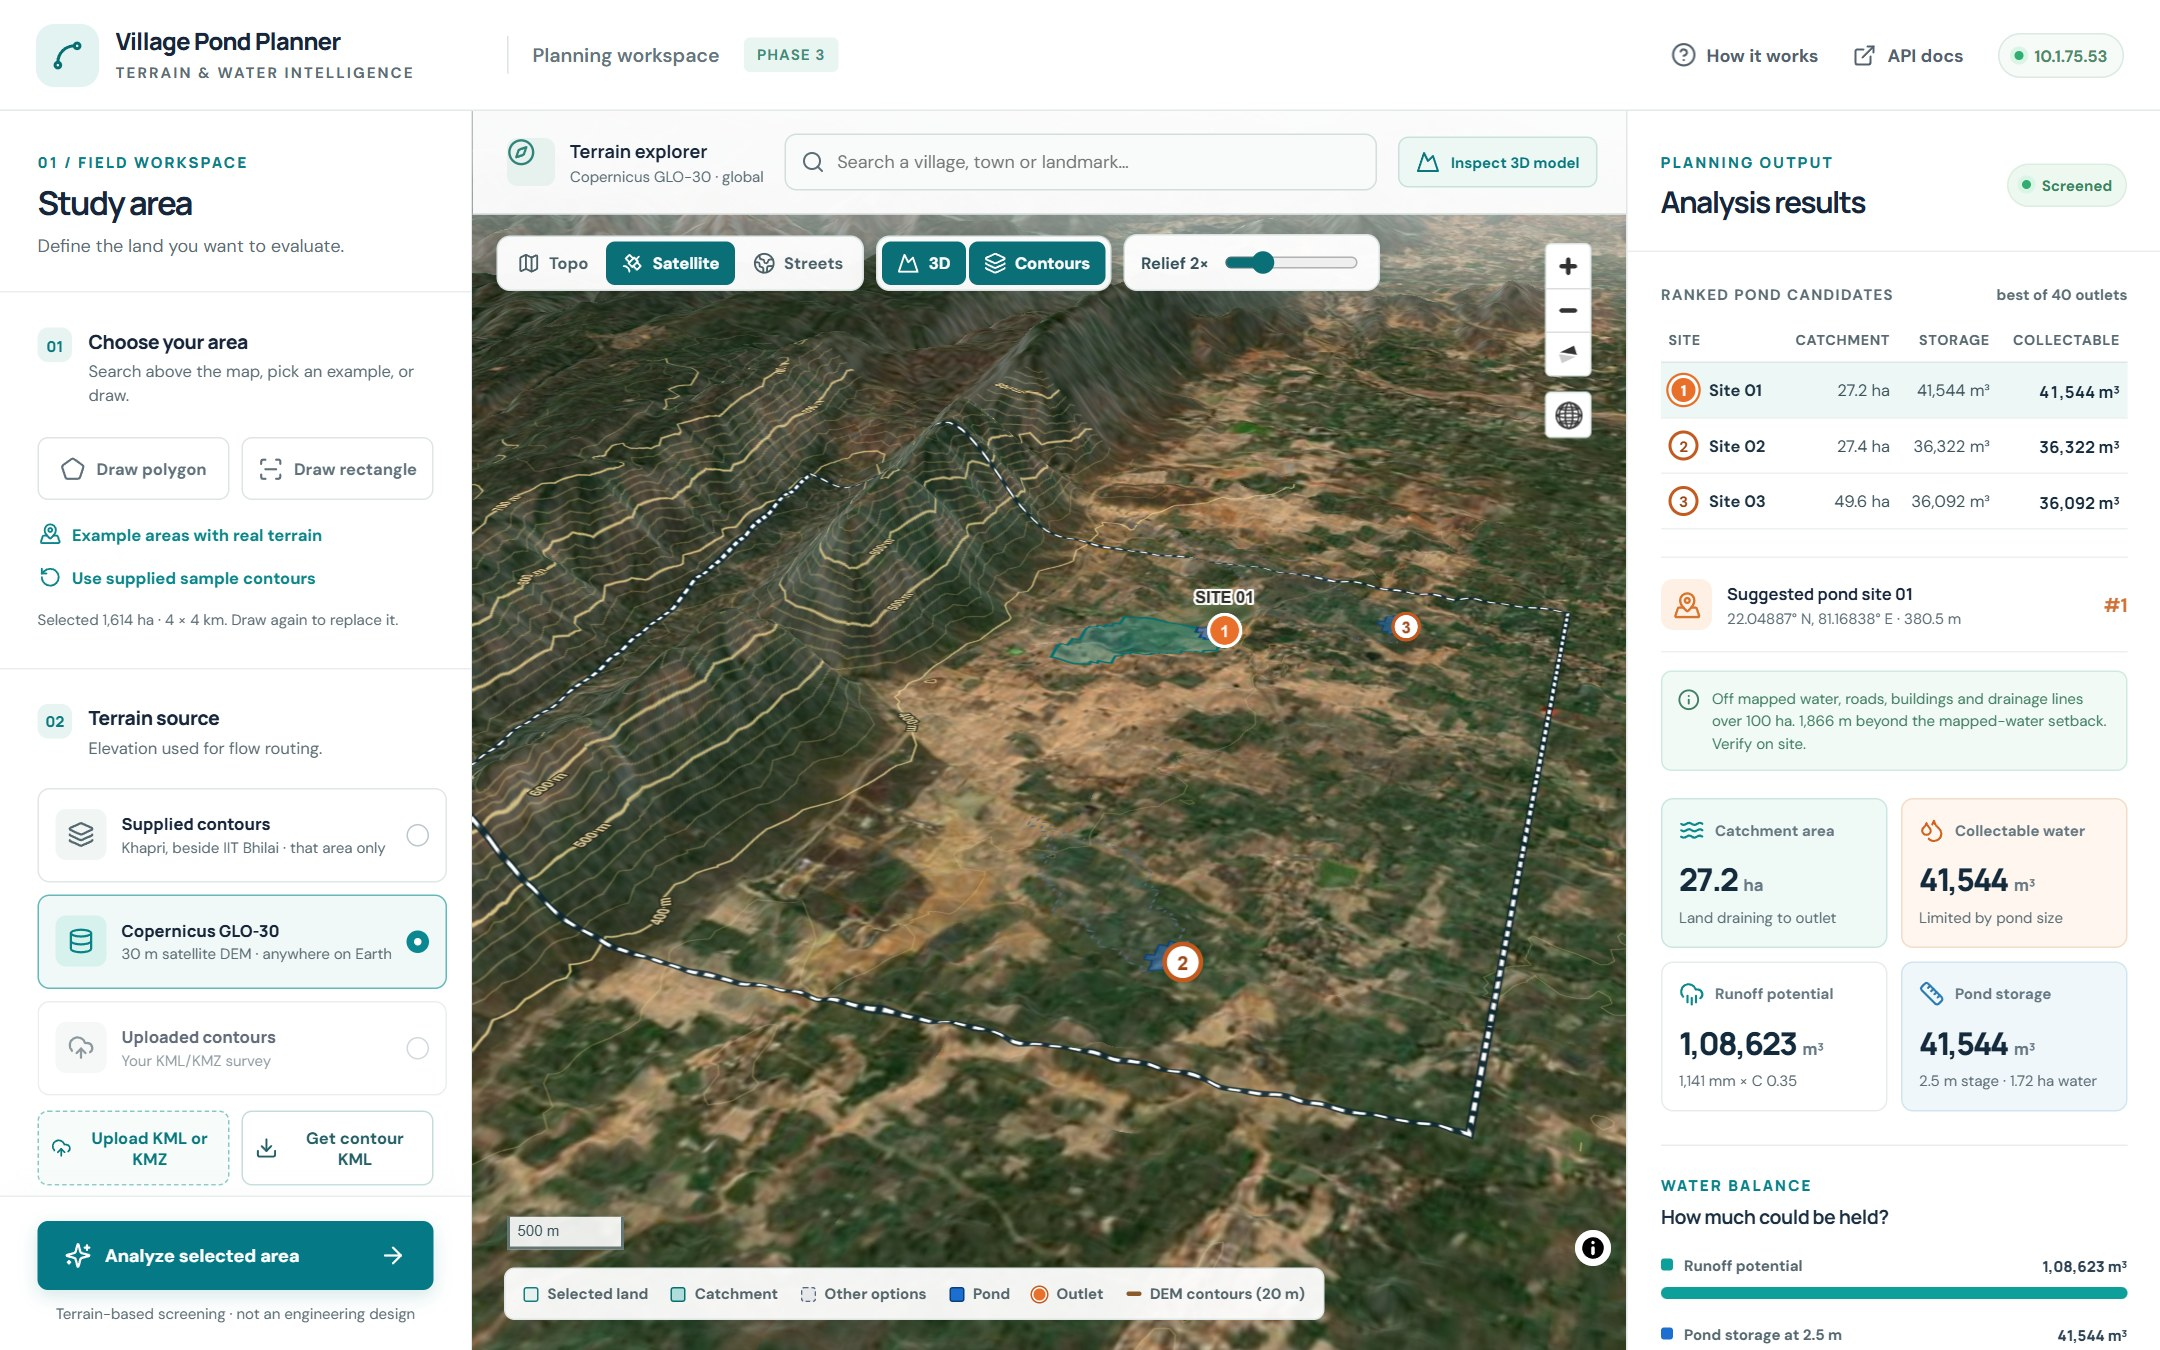
\includegraphics[width=\linewidth]{r05-3d-satellite.jpg}\par
{\footnotesize\textcolor{muted}{Live screenshot of the deployed planner: three ranked pond sites on the Maikal ridge front (Kabirdham), shown over Sentinel-2 imagery on 3D terrain.}\par}
\vspace{5mm}
{\fontsize{27}{31}\selectfont\bfseries\textcolor{navy}{AI-based Village\\Pond Planning System}\par}
\vspace{2mm}
{\large\textcolor{muted}{An interactive web planner that finds pond sites, their catchments and the water they could hold, for any area on Earth}\par}
\vspace{6mm}

\begin{tabularx}{\linewidth}{@{}Y|Y|Y@{}}
\textcolor{muted}{\footnotesize\bfseries DEPLOYMENT} & \textcolor{muted}{\footnotesize\bfseries VALIDATION} & \textcolor{muted}{\footnotesize\bfseries COVERAGE}\\
\textcolor{navy}{\large Live on the IIT network} & \textcolor{navy}{\large 34 automated tests} & \textcolor{navy}{\large 11 verified areas}\\
\textcolor{muted}{\small verified 28 Sep 2026} & \textcolor{muted}{\small pass locally and on the server} & \textcolor{muted}{\small India and Ethiopia, 60\textdegree S--60\textdegree N}\\
\end{tabularx}

\vfill
\begin{tabularx}{\linewidth}{@{}L{34mm}Y@{}}
\textcolor{muted}{\small\bfseries PLANNER} & \textbf{\url{http://10.1.75.53:3233/}} \textcolor{muted}{\small(IIT Bhilai network or VPN)}\\
\textcolor{muted}{\small\bfseries API DOCS} & \url{http://10.1.75.53:3233/docs}\\
\textcolor{muted}{\small\bfseries PHASE 2 ROUTE} & \url{http://10.1.75.53:3233/analyzeContour} (multipart field \code{contour\_map})\\
\textcolor{muted}{\small\bfseries SOURCE CODE} & \url{https://github.com/Galabavamsi/ai-village-pond-planning}\\
\textcolor{muted}{\small\bfseries AI USE} & Disclosed in Section~\ref{sec:ai}\\
\end{tabularx}
\vspace{3mm}

\textcolor{muted}{\small Prepared for the Phase 3 submission \hfill 28 September 2026}
\newpage

\tableofcontents
\newpage

% ------------------------------------------------------------------ 1
\section{Executive summary}
Phase 2 delivered an API that turns an uploaded contour map into pond-site and catchment estimates. Phase 3 turns it into a complete planning tool that an administrator can use in a browser. They select land on a map, and the planner overlays three ranked pond sites. Each site comes with its upstream catchment, the water an embankment there could hold, and the runoff that a real rainfall record would deliver.

\begin{keybox}[title=What Phase 3 delivers]
\begin{itemize}
\item \textbf{Any area, real data.} The planner uses the supplied contour map, any uploaded KML/KMZ contour map, or the global Copernicus GLO-30 elevation model anywhere between 60\textdegree S and 60\textdegree N. Rainfall comes from CHIRPS~v3 for a single month, the June--September monsoon or a full year. OpenStreetMap supplies water bodies, roads and buildings to avoid.
\item \textbf{A physically consistent pond model.} Storage counts only land that drains to the pond outlet and lies below the embankment crest. Sites are ranked by the water they could actually collect. Each site reports a stage--storage curve, an indicative embankment length and warnings.
\item \textbf{Earth view.} The map offers topographic, Sentinel-2 satellite and street basemaps, labelled contours, 3D terrain, a globe view, and a 3D model of the exact analysis grid with an optional satellite drape. Results export to Google Earth KML, GeoJSON and contour KML.
\item \textbf{Deployed and verified.} The planner runs on the assigned IIT container. All 34 tests pass there. The browser test suites pass against the live address, from the campus network.
\end{itemize}
\end{keybox}

Before this final build, the Phase 3 prototype was reviewed line by line. The review found and fixed four defects that changed results:
\begin{itemize}
\item pond storage was inflated by 37--272\,\%;
\item site ranking ignored storage;
\item map screening failed for larger areas;
\item the map lost the selected area when the terrain source changed.
\end{itemize}
A later check found and fixed a fifth: flat terraces created when coarse contours are interpolated. These defects are documented in Section~\ref{sec:review}.

\begin{warnbox}[title=Honest scope]
All numbers are deterministic screening estimates computed from gridded elevation and historical rainfall. They are not an engineering design, a hydrological simulation or a land-eligibility decision. No language model computes any result. Seepage, evaporation, siltation, soil, spillway design and land ownership are not modelled, and the planner says so in every result.
\end{warnbox}

% ------------------------------------------------------------------ 2
\clearpage
\section{Requirements and traceability}
\begin{tabularx}{\linewidth}{@{}L{42mm}YL{17mm}@{}}
\toprule
\textbf{Phase 3 requirement} & \textbf{Implementation and evidence} & \textbf{Status}\\
\midrule
Select land on a map & Draw a polygon or rectangle (Terra Draw), pick one of 11 example areas, or search any place (Photon/OSM). The area and span are shown live and validated (0.25--10,000~ha, $\leq$20~km). Figs.~\ref{fig:sample}, \ref{fig:examples}. & Done\\
Analyze the land & \code{POST /api/analyze-area} with the supplied, uploaded or Copernicus elevation, CHIRPS or manual rainfall, and land-cover and pond settings (Section~\ref{sec:algorithms}). & Done\\
Show pond location, catchment and water volume on the map & Numbered outlets, pond polygons and catchment polygons for all three sites (active one highlighted), plus runoff, storage and collectable volume, a stage--storage chart and benchmarks (Figs.~\ref{fig:sample}, \ref{fig:panel}). & Done\\
Works beyond the sample & Copernicus GLO-30 anywhere at 60\textdegree S--60\textdegree N. Ten areas outside the sample were verified end to end (Section~\ref{sec:examples}). & Done\\
No hard-coded results & All inputs come from the selected polygon and data source. The example list only moves the map. A test uploads and analyzes every shipped KML. & Done\\
Front end on the IIT system & \url{http://10.1.75.53:3233/} on sys1 (SSH port 2233, Application~1 port), verified from the campus network (Section~\ref{sec:deploy}). & Done\\
Phase 2 API compatibility & \code{POST /analyzeContour} (field \code{contour\_map}) and \code{/findCatchment} unchanged; Phase 2 tests pass. & Done\\
GitHub repository & \url{https://github.com/Galabavamsi/ai-village-pond-planning}, branch \code{master}. & Done\\
Report and demo video & This report; the video follows the walkthrough in Appendix~\ref{app:demo}. & Report done\\
\bottomrule
\end{tabularx}

% ------------------------------------------------------------------ 3
\section{System architecture}
The planner is one FastAPI application that serves both the API and the compiled React front end, so there is a single origin and a single process to run. Figure~\ref{fig:architecture} shows the parts and the data they use.

\begin{figure}[htbp]
\centering
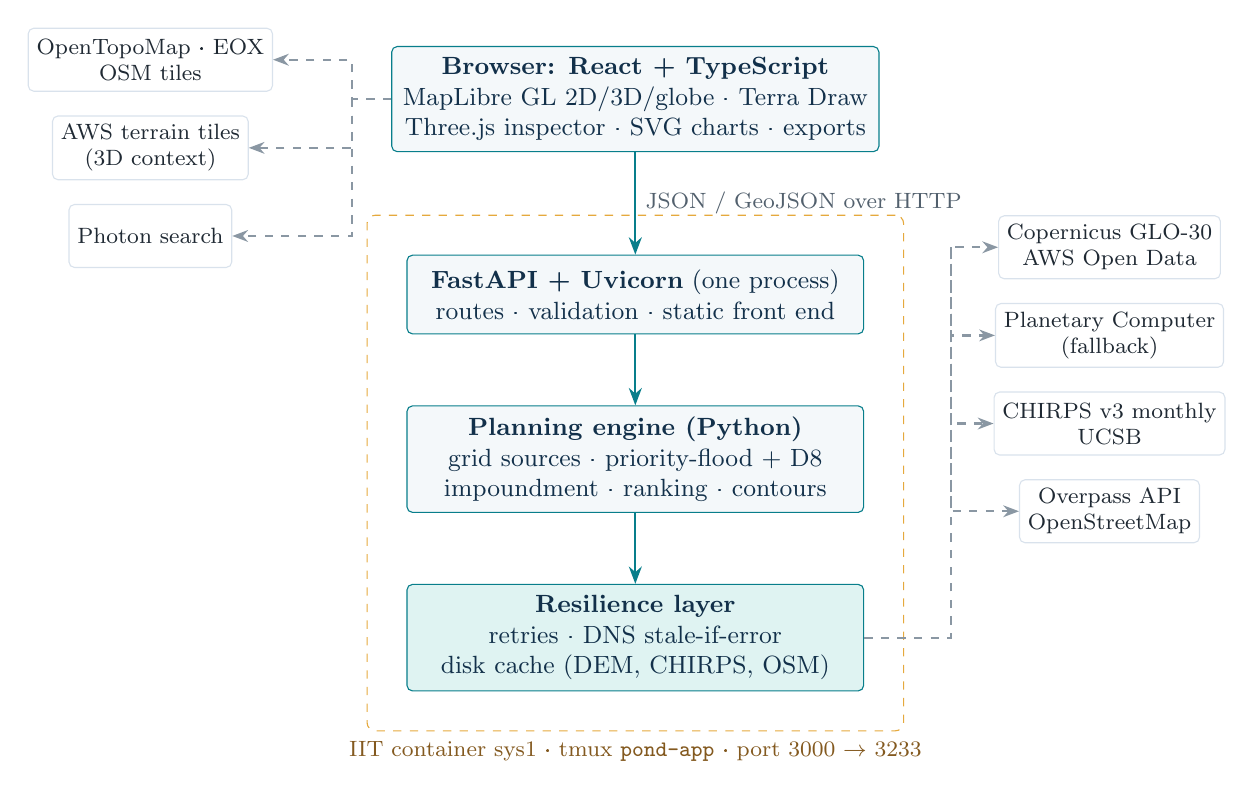
\begin{tikzpicture}[
  font=\small,
  box/.style={draw=teal,rounded corners=2pt,fill=pale,align=center,text=navy,minimum height=10mm,inner sep=4pt},
  ext/.style={draw=line,rounded corners=2pt,fill=white,align=center,text=ink,minimum height=8mm,font=\footnotesize,inner sep=3pt},
  arrow/.style={-{Stealth[length=2.2mm]},thick,teal},
  remote/.style={-{Stealth[length=2mm]},thick,old,dashed}]
\node[box,minimum width=58mm] (ui) {\textbf{Browser: React + TypeScript}\\MapLibre GL 2D/3D/globe \textperiodcentered{} Terra Draw\\Three.js inspector \textperiodcentered{} SVG charts \textperiodcentered{} exports};
\node[box,minimum width=58mm,below=13mm of ui] (api) {\textbf{FastAPI + Uvicorn} (one process)\\routes \textperiodcentered{} validation \textperiodcentered{} static front end};
\node[box,minimum width=58mm,below=9mm of api] (engine) {\textbf{Planning engine (Python)}\\grid sources \textperiodcentered{} priority-flood + D8\\impoundment \textperiodcentered{} ranking \textperiodcentered{} contours};
\node[box,minimum width=58mm,below=9mm of engine,fill=mint] (cache) {\textbf{Resilience layer}\\retries \textperiodcentered{} DNS stale-if-error\\disk cache (DEM, CHIRPS, OSM)};
\node[ext,right=17mm of api,yshift=6mm] (aws) {Copernicus GLO-30\\AWS Open Data};
\node[ext,below=3mm of aws] (pc) {Planetary Computer\\(fallback)};
\node[ext,below=3mm of pc] (chirps) {CHIRPS v3 monthly\\UCSB};
\node[ext,below=3mm of chirps] (overpass) {Overpass API\\OpenStreetMap};
\node[ext,left=15mm of ui,yshift=5mm] (tiles) {OpenTopoMap \textperiodcentered{} EOX\\OSM tiles};
\node[ext,below=3mm of tiles] (terrain) {AWS terrain tiles\\(3D context)};
\node[ext,below=3mm of terrain] (photon) {Photon search};
\draw[arrow] (ui) -- node[right,font=\footnotesize,text=muted]{JSON / GeoJSON over HTTP} (api);
\draw[arrow] (api) -- (engine);
\draw[arrow] (engine) -- (cache);
\draw[remote] (cache.east) -| ($(aws.west)+(-6mm,0)$) -- (aws.west);
\draw[remote] ($(aws.west)+(-6mm,0)$) |- (pc.west);
\draw[remote] ($(aws.west)+(-6mm,0)$) |- (chirps.west);
\draw[remote] ($(aws.west)+(-6mm,0)$) |- (overpass.west);
\draw[remote] (ui.west) -- ++(-5mm,0) |- (tiles.east);
\draw[remote] (ui.west) ++(-5mm,0) |- (terrain.east);
\draw[remote] (ui.west) ++(-5mm,0) |- (photon.east);
\begin{scope}[on background layer]
\node[draw=gold,dashed,rounded corners=3pt,fit=(api)(engine)(cache),inner sep=5mm,label={[text=warnfg,font=\footnotesize]south:IIT container sys1 \textperiodcentered{} tmux \code{pond-app} \textperiodcentered{} port 3000 $\rightarrow$ 3233}] {};
\end{scope}
\end{tikzpicture}
\caption{Architecture. Solid arrows are the planner's own calls. Dashed arrows are remote data sources: the browser loads map tiles, terrain tiles and search itself, and the server reads elevation, rainfall and OSM features. Each server-side source is retried and cached.}
\label{fig:architecture}
\end{figure}

\begin{tabularx}{\linewidth}{@{}L{30mm}Y@{}}
\toprule
\textbf{Layer} & \textbf{Technology (version)}\\
\midrule
Front end & React 19, TypeScript 5.9, Vite 7, MapLibre GL JS 6.11 (globe, terrain, sky), Terra Draw 1.35, Three.js 0.186, lucide icons\\
API & FastAPI 0.141, Uvicorn, Pydantic request models, OpenAPI/Swagger at \code{/docs}\\
Geospatial & NumPy 2.5, SciPy 1.18 (interpolation, morphology), Shapely 2.1, rasterio 1.5 with GDAL 3.12, contourpy 1.4, pystac-client, planetary-computer\\
Testing & pytest (34 tests), Playwright with installed Chrome (desktop and mobile browser suites)\\
Hosting & Ubuntu 24.04 container on the IIT system, Python 3.12 virtual environment, tmux supervision\\
\bottomrule
\end{tabularx}

% ------------------------------------------------------------------ 4
\section{Features and user workflow}
\label{sec:features}

\subsection{Choosing land anywhere}
The workspace has three columns: the study-area controls, the map, and the results (Figure~\ref{fig:sample}). A planner can:
\begin{itemize}
\item \textbf{draw} a polygon or rectangle on the map;
\item \textbf{search} a village, town or landmark, which selects a 2\,km square around it (Figure~\ref{fig:search});
\item \textbf{pick an example area} with real terrain (Figure~\ref{fig:examples}).
\end{itemize}
The panel shows the selected area and its width and height in kilometres live, and rejects impossible sizes before any request is sent. Drawing outside the supplied or uploaded contours switches the terrain source to Copernicus GLO-30 automatically and explains why in a notice.

\begin{figure}[htbp]
\centering
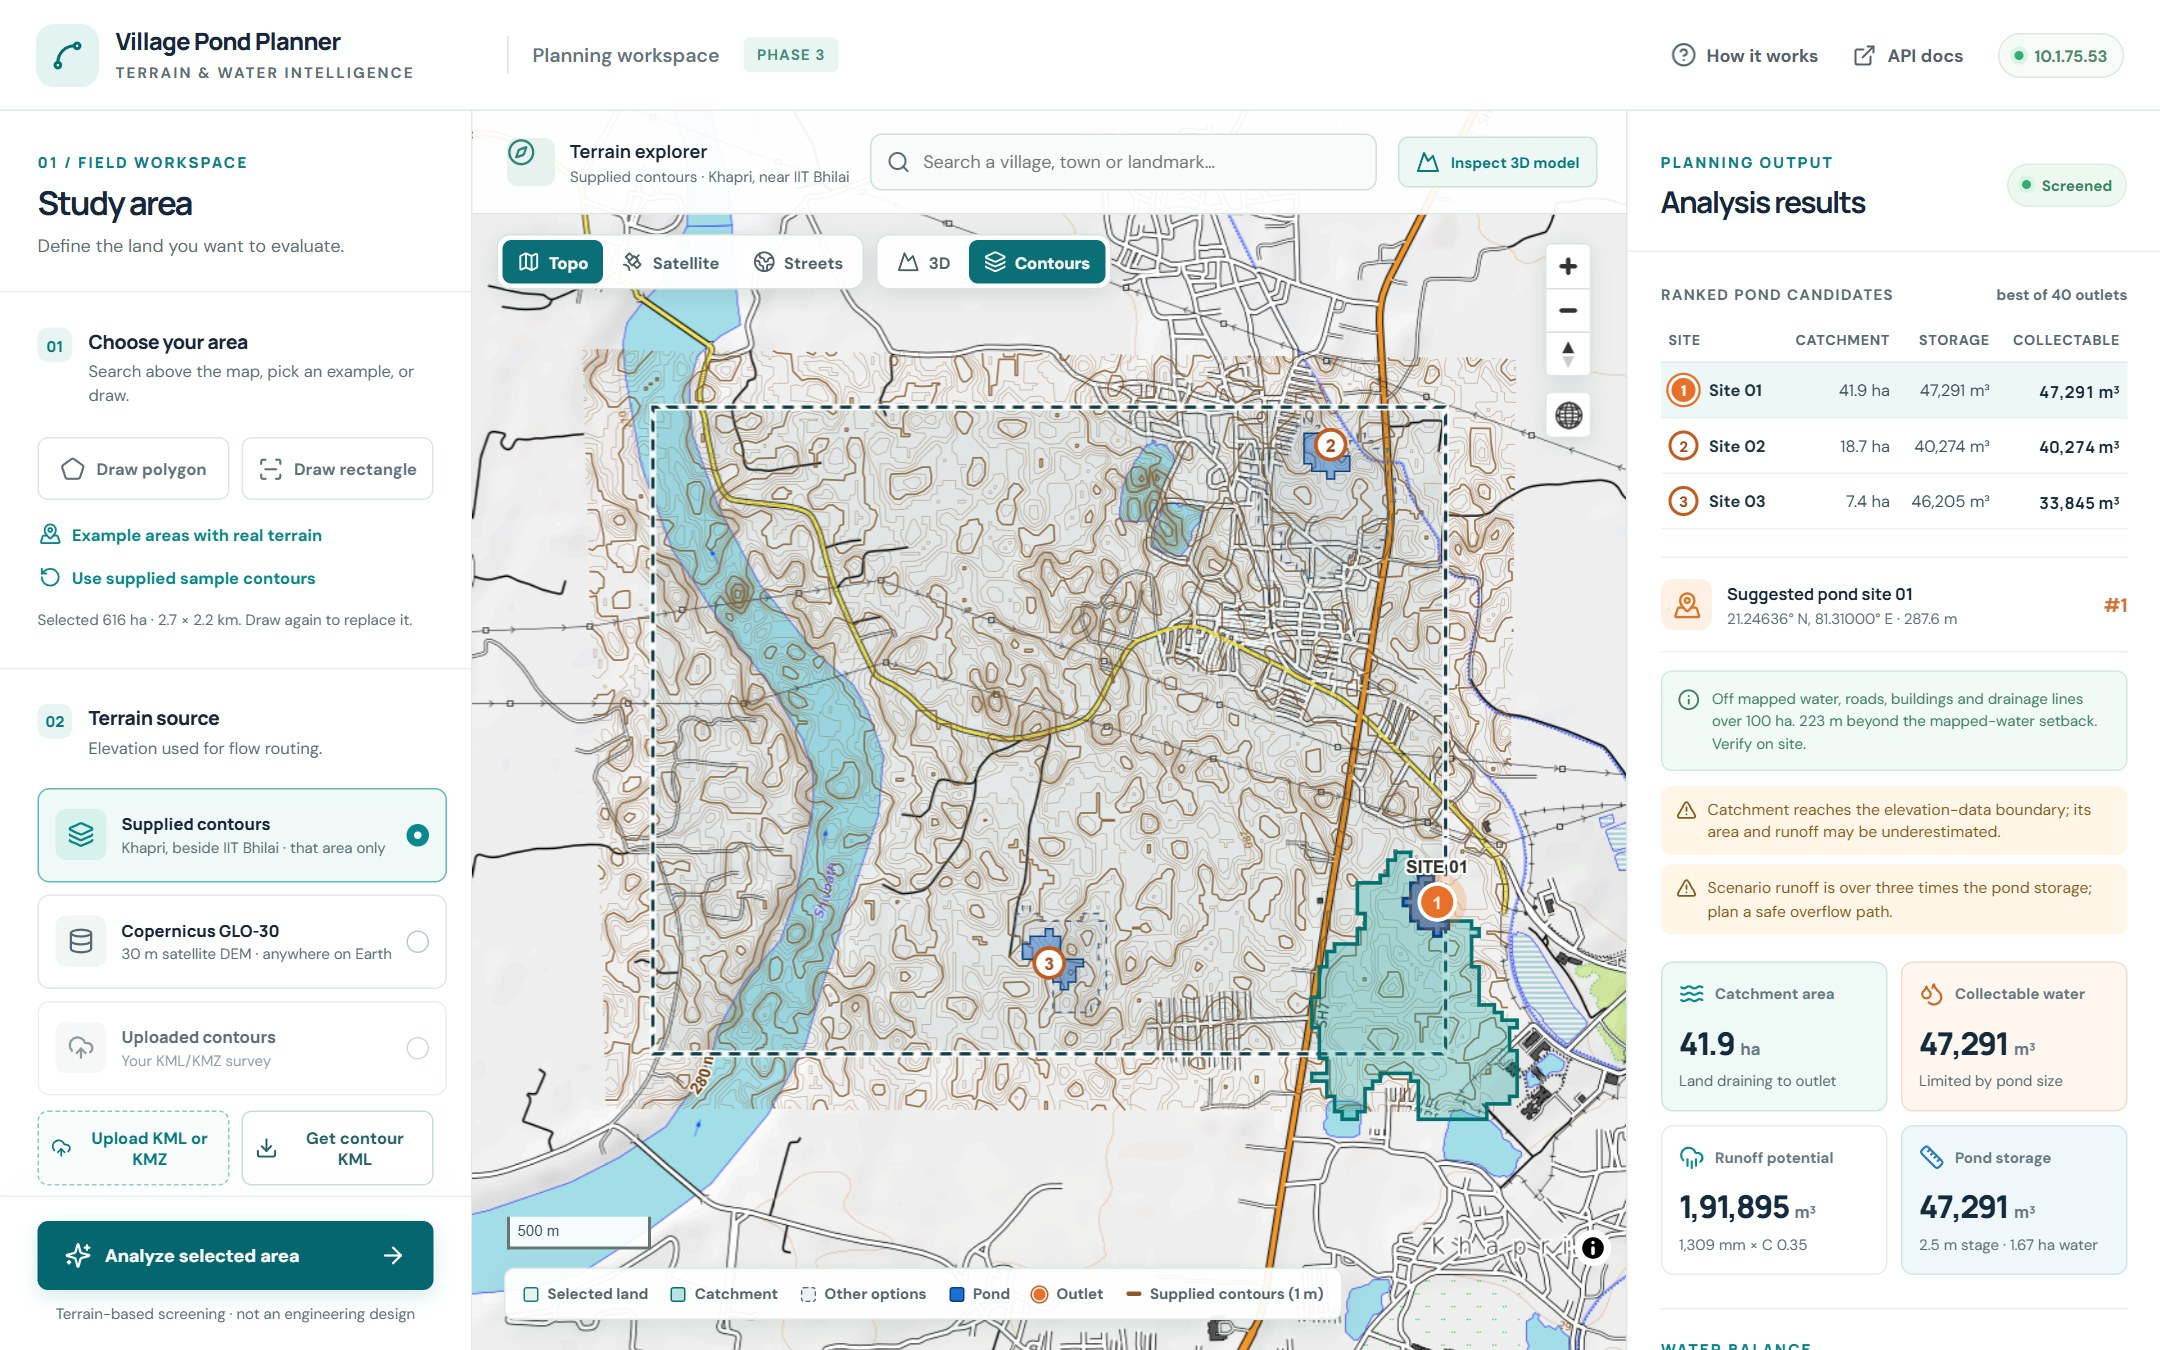
\includegraphics[width=\linewidth]{r01-sample-results.jpg}
\caption{Supplied contour map (Khapri, beside IIT Bhilai) analyzed with the June--September 2025 CHIRPS rainfall. Three numbered outlets, their ponds (blue) and catchments (teal for the active site, dashed grey for the alternatives) sit over the labelled 1\,m contours. The results column ranks the sites by collectable water and lists warnings. The header badge shows the live host 10.1.75.53.}
\label{fig:sample}
\end{figure}

\begin{figure}[htbp]
\centering
\begin{subfigure}[t]{0.49\linewidth}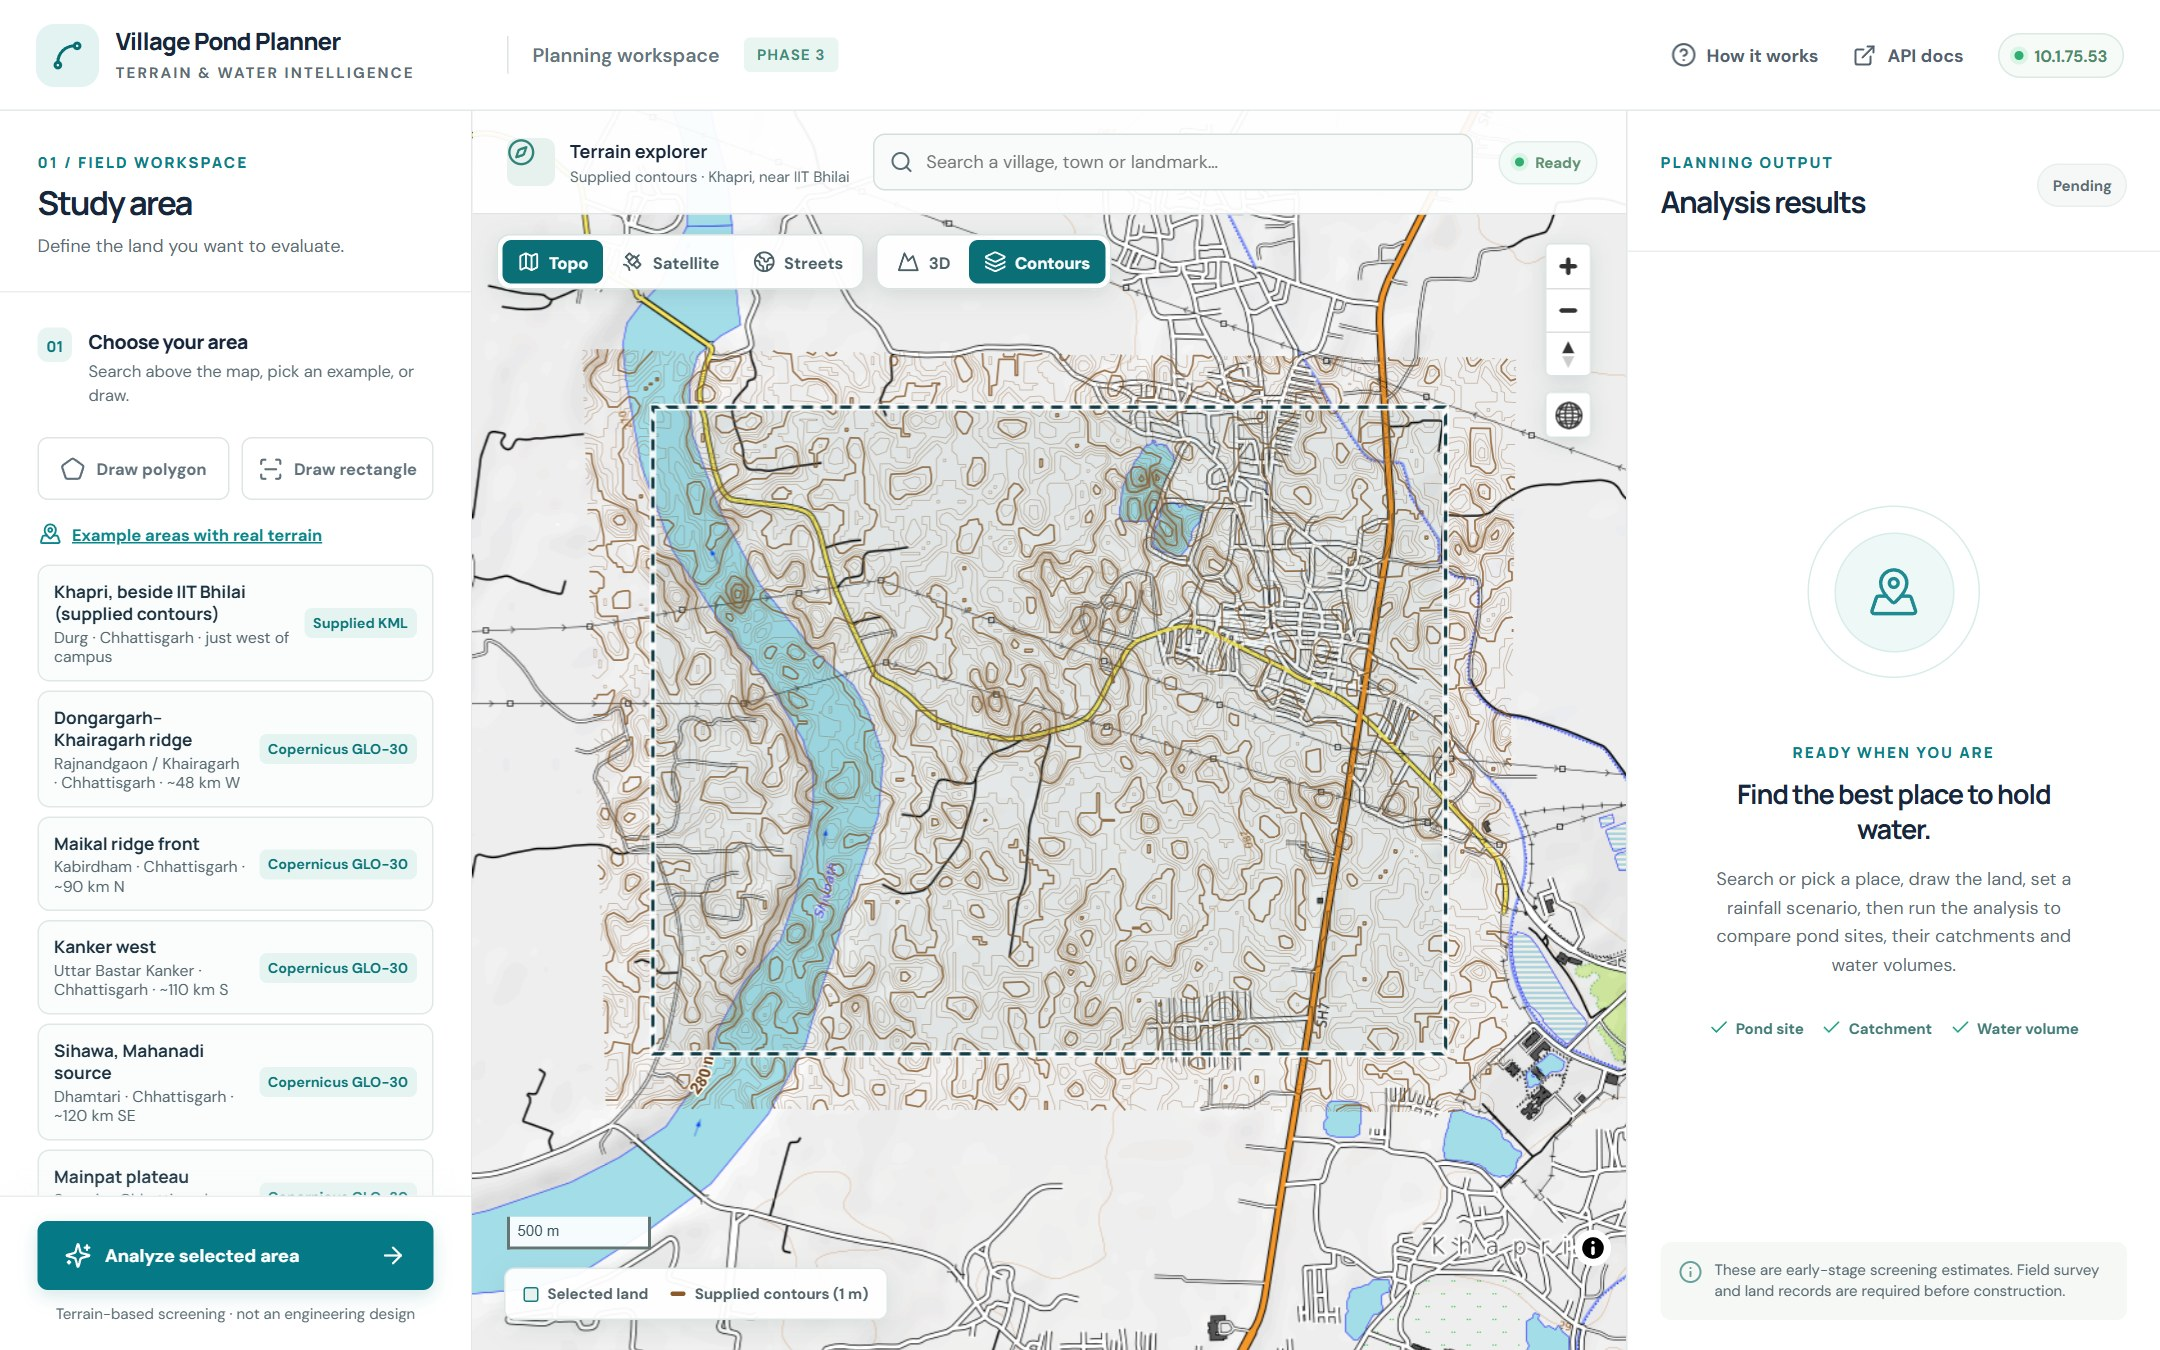
\includegraphics[width=\linewidth]{r02-examples.jpg}\caption{Example areas with real terrain.}\label{fig:examples}\end{subfigure}\hfill
\begin{subfigure}[t]{0.49\linewidth}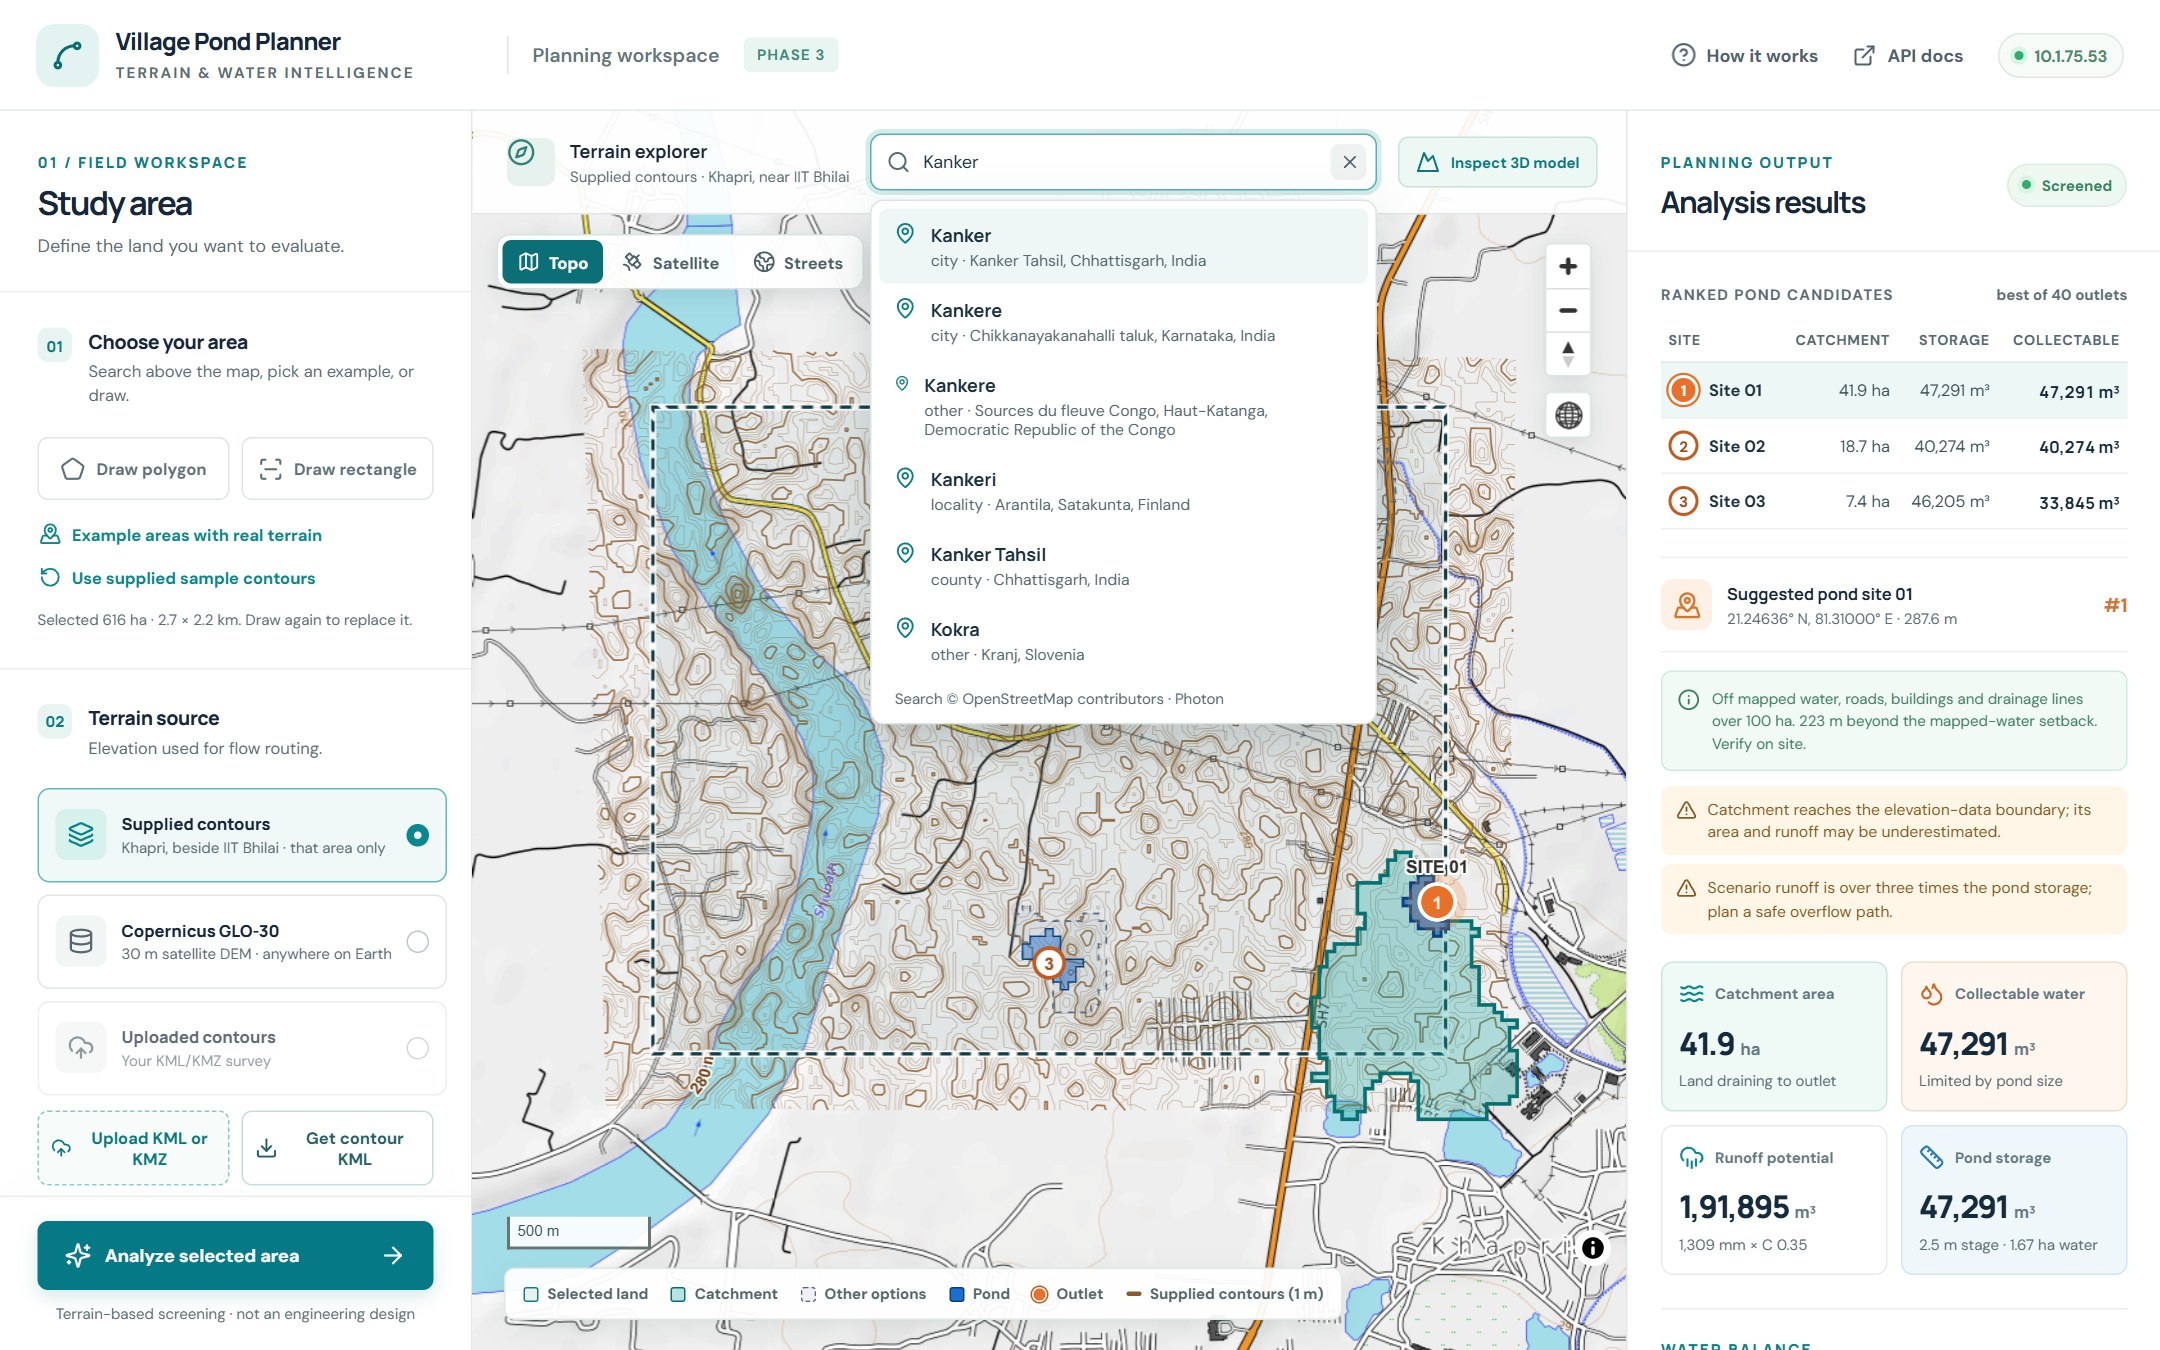
\includegraphics[width=\linewidth]{r03-search.jpg}\caption{Place search (Photon, OpenStreetMap data).}\label{fig:search}\end{subfigure}
\caption{Two quick ways to reach an area other than the sample.}
\end{figure}

\subsection{Terrain sources}
\begin{itemize}
\item \textbf{Supplied contours:} the course KML (2,710 lines, 267--298\,m). Section~\ref{sec:data} explains its provenance.
\item \textbf{Uploaded contours:} any KML or KMZ up to 20\,MB. Each line's elevation is read from its placemark name, an \code{ExtendedData} field (\code{elevation}, \code{elev}, \code{z}, \code{height} or \code{level}), or a constant coordinate altitude. The uploaded linework is drawn on the map (Figure~\ref{fig:upload}).
\item \textbf{Copernicus GLO-30:} a 30\,m global surface model, read for the selected area plus a buffer, so catchments can extend beyond the drawn land.
\item \textbf{Get contour KML:} traces real contours for \emph{any} selected area. The file opens in Google Earth and can be uploaded back as a contour survey.
\end{itemize}

\begin{figure}[htbp]
\centering
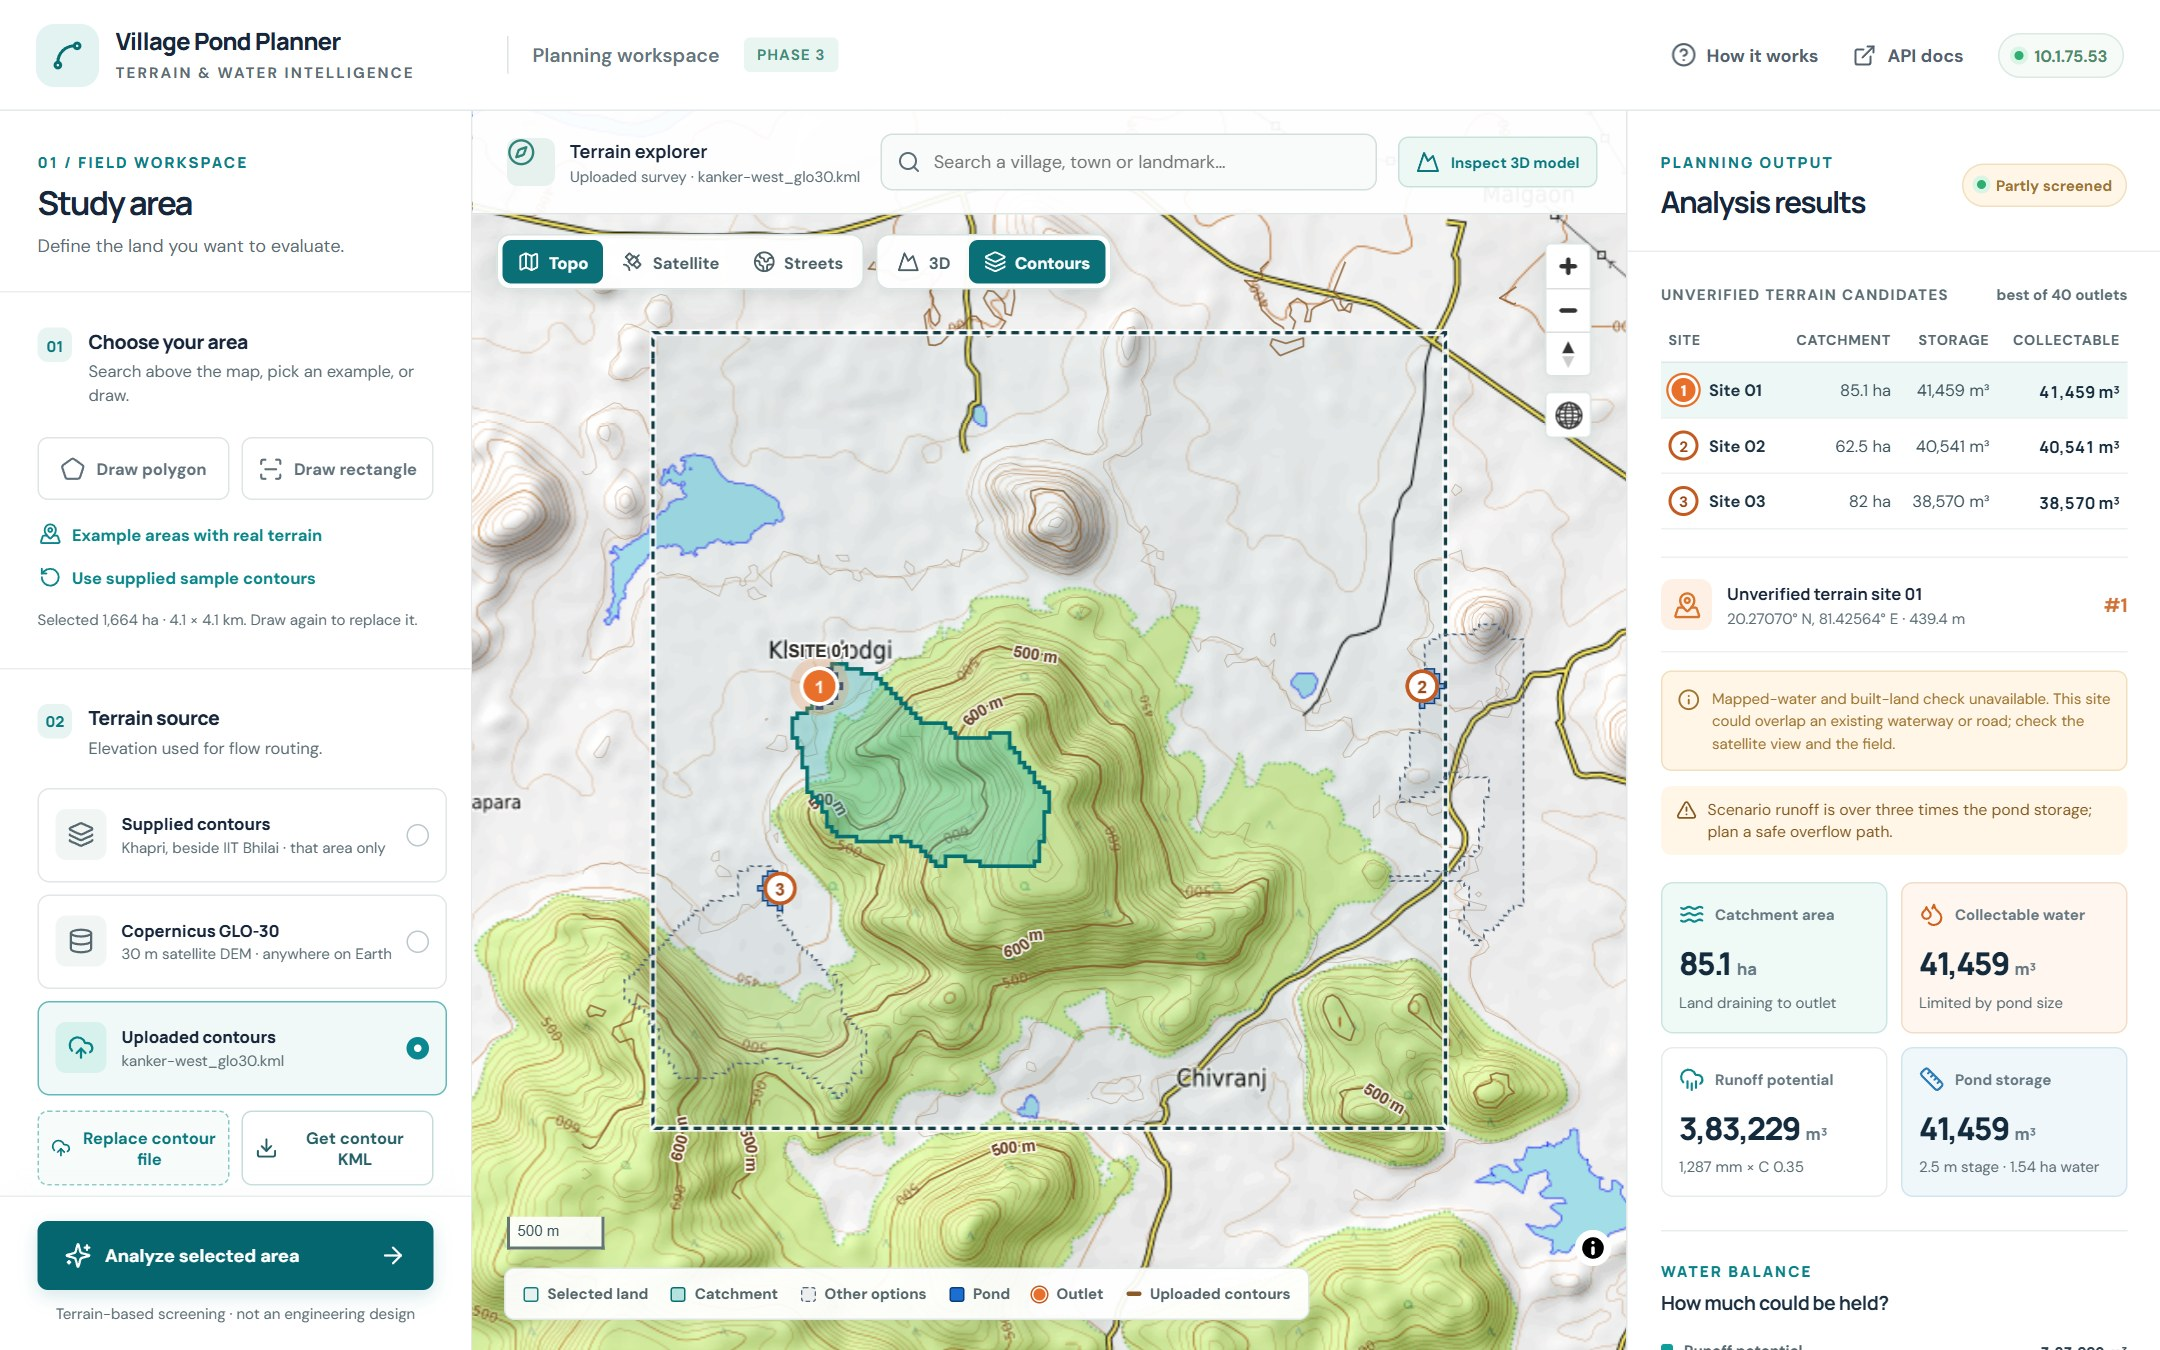
\includegraphics[width=0.92\linewidth]{r11-upload-results.jpg}
\caption{A real GLO-30-derived contour KML for Kanker west, uploaded and analyzed on the live server. The three outlets drain different valleys. During this run the server could not reach Overpass for this new area, so the result is honestly labelled ``Partly screened'' and ``unverified terrain candidates''; it is not presented as cleared land.}
\label{fig:upload}
\end{figure}

\subsection{Rainfall, land cover and pond settings}
CHIRPS~v3 provides a historical monthly rainfall total on a 0.05\textdegree{} grid. The planner can use one month, the June--September season (the Indian south-west monsoon, when most runoff occurs) or a calendar year. Only completed months are offered. Alternatively the user enters a rainfall depth. The runoff coefficient has land-cover presets within the ranges of the CGWB \emph{Manual on Artificial Recharge}~[\ref{ref:cgwb}] (Table~\ref{tab:presets}). The water stage (embankment height, 0.5--6\,m) sets the pond size. An advanced setting caps the catchment treated as a ``small pond'' at 100\,ha by default.

\begin{table}[htbp]
\centering\small
\begin{tabular}{@{}lcl@{}}
\toprule
\textbf{Preset} & \textbf{$C$} & \textbf{Basis (CGWB manual)}\\
\midrule
Forest & 0.15 & tree cover, volumetric range 0.05--0.2\\
Paddy & 0.20 & flat bunded cropland; Barlow 10--20\,\%\\
Scrub & 0.25 & grass, scrub and fallow land\\
Hilly & 0.35 & hills and plains with little cultivation; Barlow 35\,\%\\
Rocky & 0.50 & bare or rocky slopes, about 0.4--0.7\\
Built-up & 0.75 & roofs, roads, paved yards\\
\bottomrule
\end{tabular}
\caption{Runoff-coefficient presets. They are seasonal fractions for screening, not peak-flow design values.}
\label{tab:presets}
\end{table}

\begin{figure}[htbp]
\centering
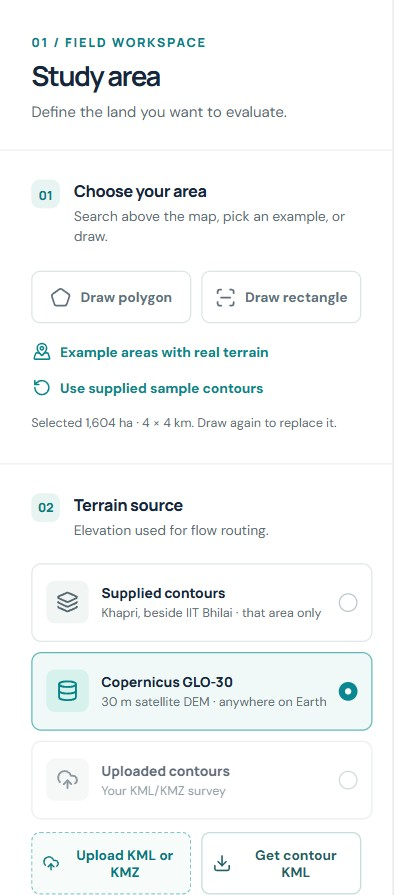
\includegraphics[width=0.3\linewidth]{r14-controls-panel-1.jpg}\hspace{8mm}
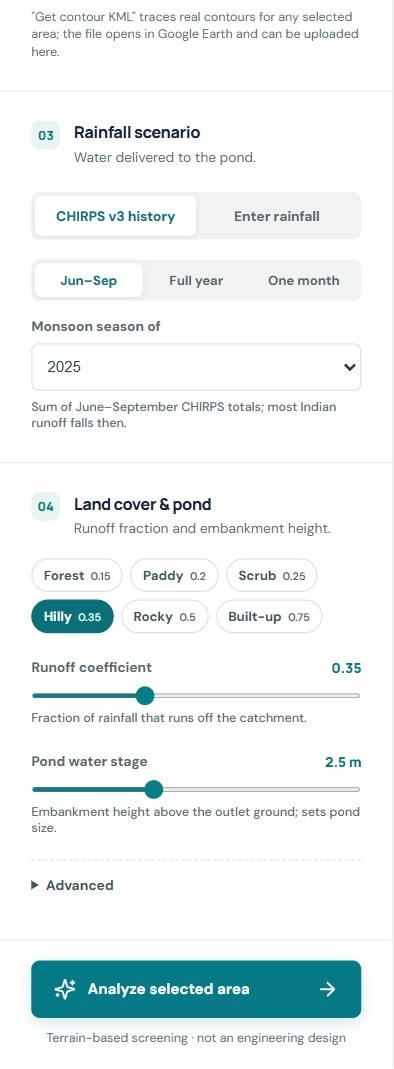
\includegraphics[width=0.3\linewidth]{r14-controls-panel-2.jpg}
\caption{The full study-area panel, split into two columns: 01 area selection with the live size check; 02 terrain source and the contour-KML export; 03 rainfall period and year; 04 land-cover presets, pond stage and the advanced catchment cap.}
\label{fig:controls}
\end{figure}

\subsection{Results, comparison and benchmarks}
The results panel (Figure~\ref{fig:panel}) supports the decision the administrator actually has to make:
\begin{itemize}
\item a \textbf{comparison table} of the three alternatives;
\item \textbf{metrics} for the active site: catchment area, collectable water (and whether runoff or pond size limits it), runoff potential and pond storage;
\item a \textbf{water balance} with bars on one shared scale;
\item \textbf{pond facts}: crest level, mean depth, indicative bund length and storage per metre of bund;
\item \textbf{benchmarks} against Mission Amrit Sarovar and MGNREGA farm-pond norms~[\ref{ref:amrit},\ref{ref:mgnrega}];
\item a \textbf{stage--storage chart} with a crosshair tooltip and a table view;
\item \textbf{monthly rainfall bars};
\item data \textbf{provenance}, and \textbf{exports}.
\end{itemize}
Each site also carries plain-language warnings: its catchment reaches the grid edge, it drains more than the small-pond cap, or runoff is more than three times, or less than half, its storage.

\begin{figure}[htbp]
\centering
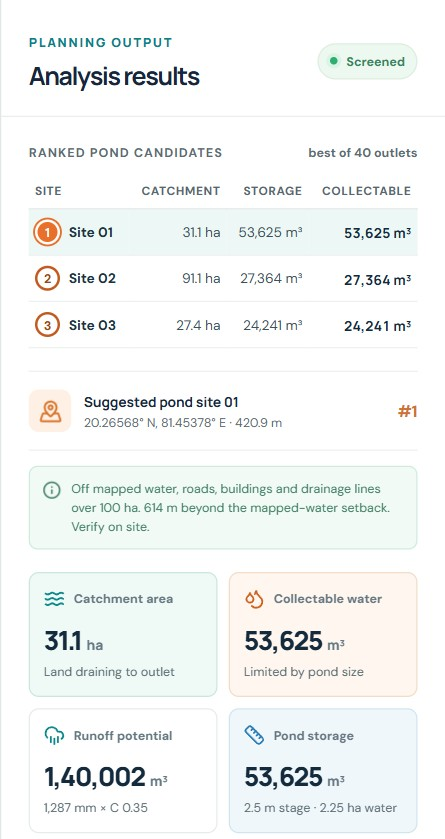
\includegraphics[width=0.32\linewidth]{r07-results-panel-1.jpg}\hfill
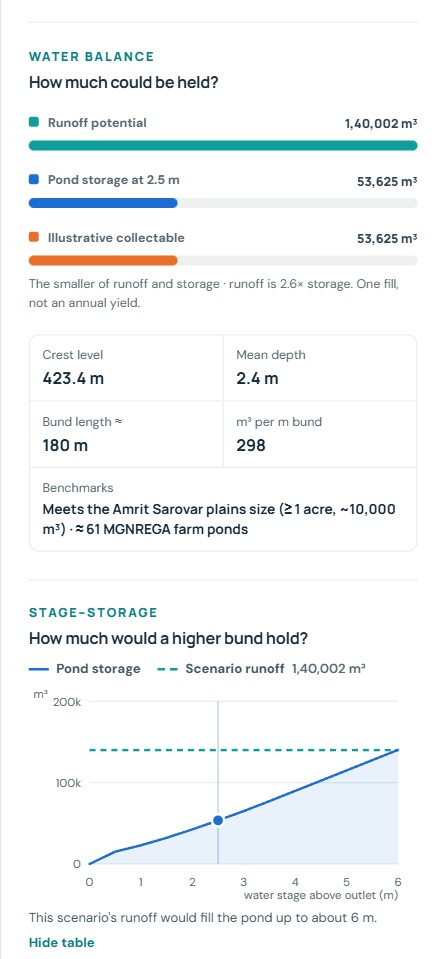
\includegraphics[width=0.32\linewidth]{r07-results-panel-2.jpg}\hfill
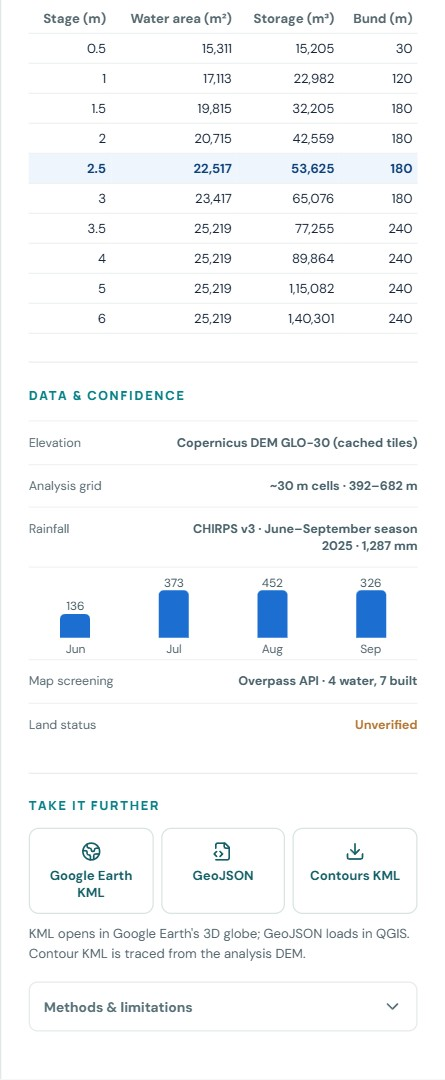
\includegraphics[width=0.32\linewidth]{r07-results-panel-3.jpg}
\caption{The complete results panel for Kanker west (live server), split into three columns. From left: ranked comparison and metrics; water balance, pond facts, benchmarks and the stage--storage chart; its table view, data provenance with the monthly CHIRPS bars, and exports.}
\label{fig:panel}
\end{figure}

\subsection{Maps, 3D terrain and globe view}
The map toolbar switches between three basemaps: OpenTopoMap topography, EOX Sentinel-2 cloudless 2025 imagery and OpenStreetMap streets. It also toggles contours and \textbf{3D}, which tilts the map over global terrain tiles with adjustable relief. The globe button zooms out to the whole Earth with an atmosphere (Figure~\ref{fig:earth}). Contours are labelled every fifth line. Before analysis they come from the survey; after a Copernicus analysis they are traced from the analysis grid. The map is created once and updated in place, so switching source or basemap never loses the selection.

\begin{figure}[htbp]
\centering
\begin{subfigure}[t]{0.49\linewidth}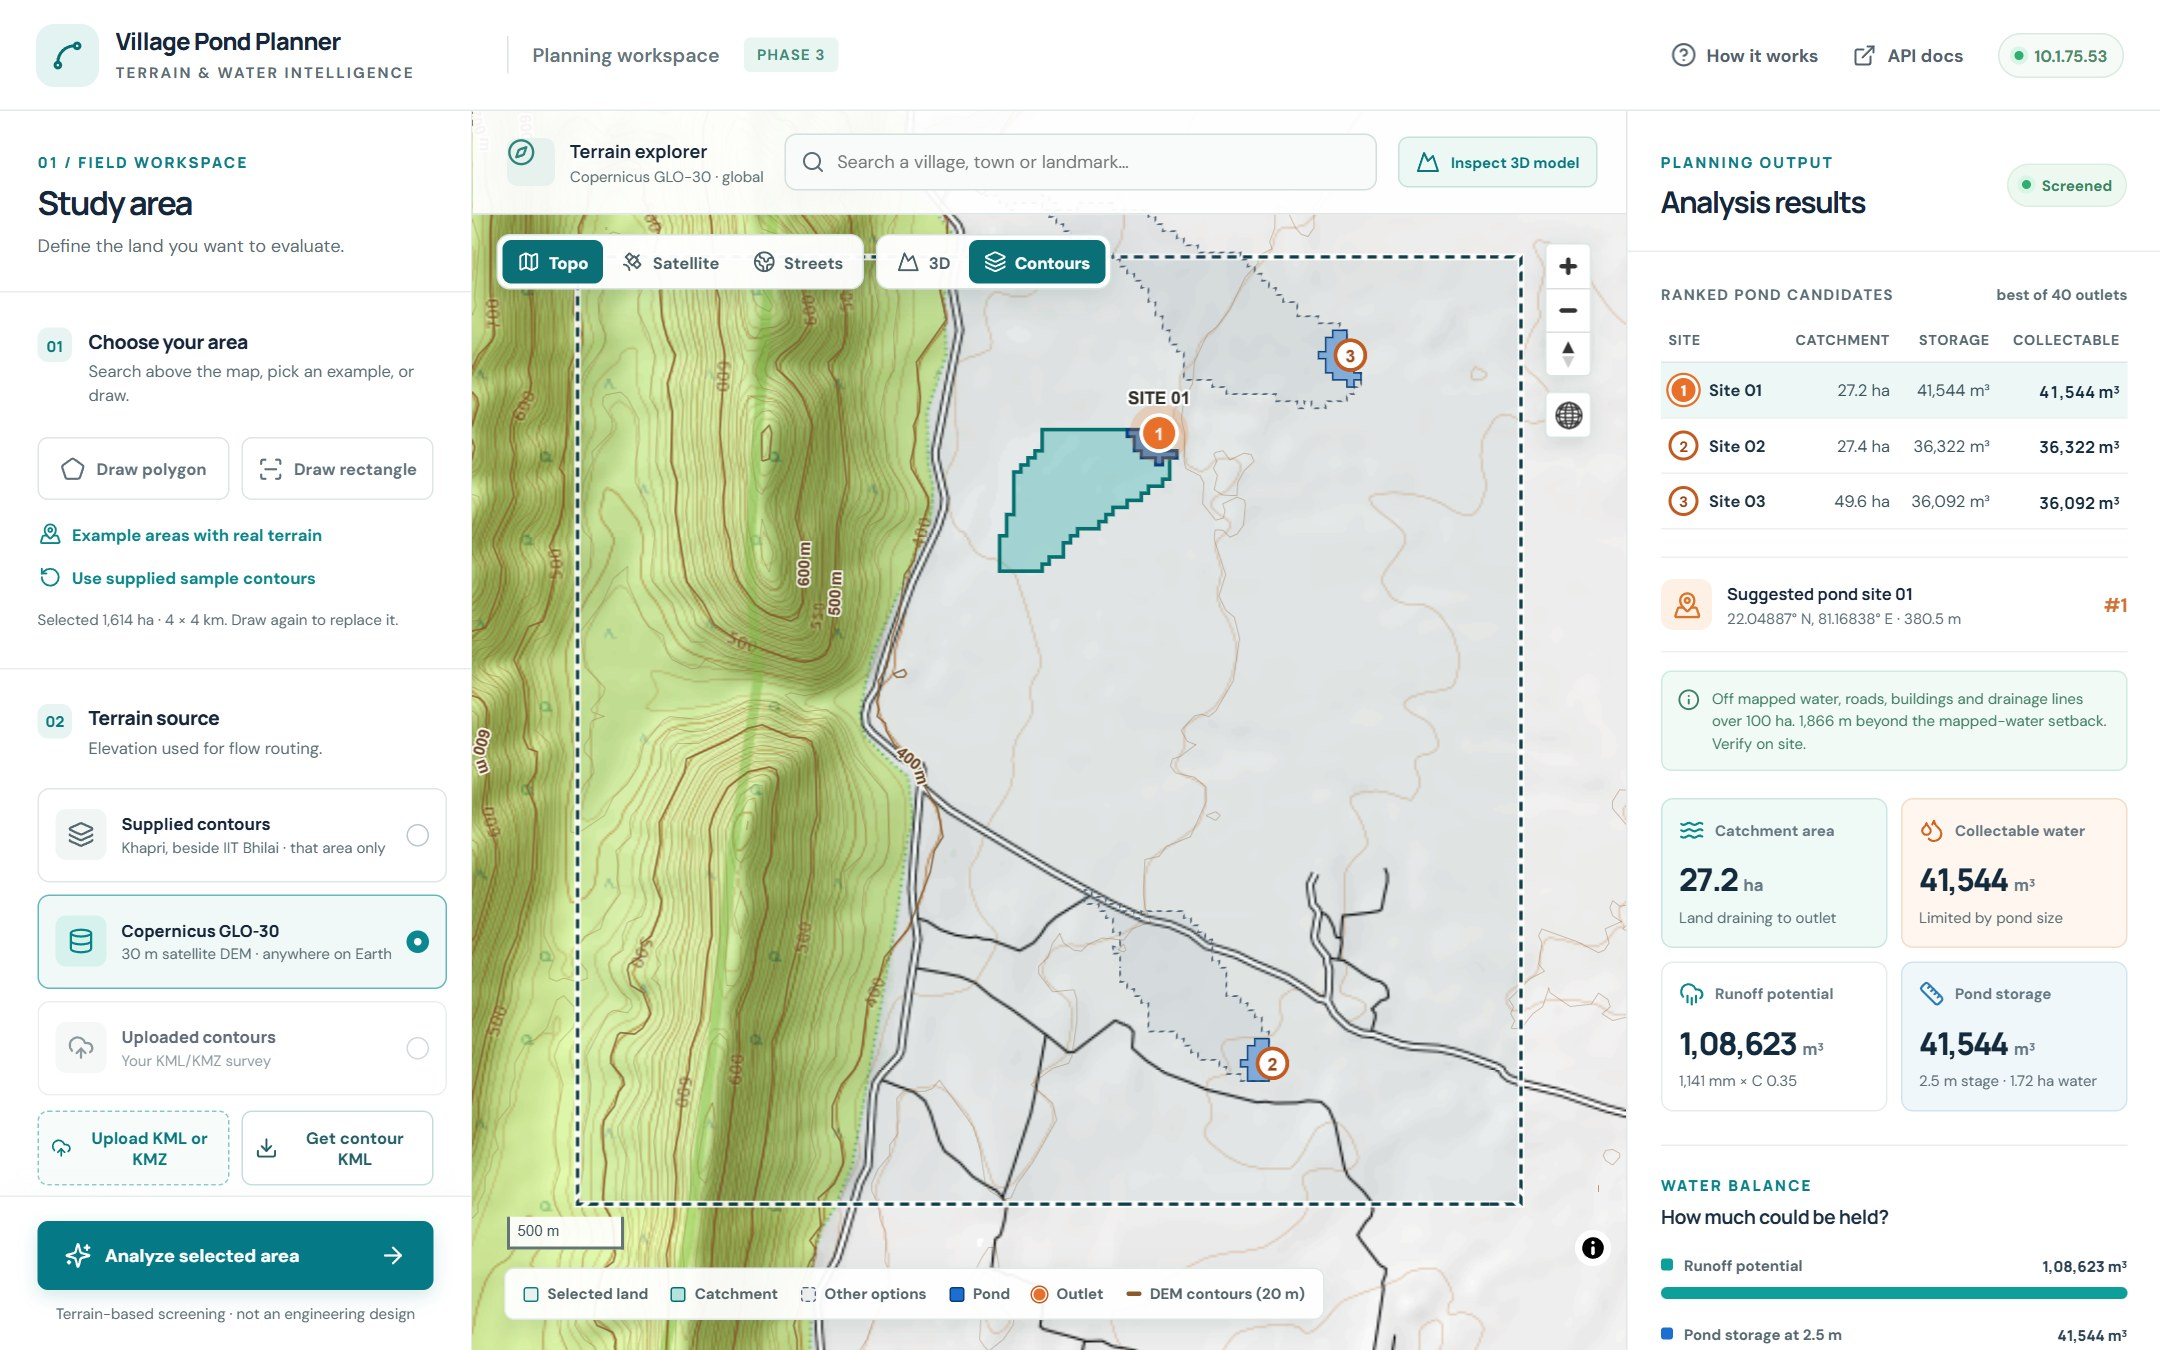
\includegraphics[width=\linewidth]{r04-example-topo.jpg}\caption{Maikal ridge front, topographic basemap with 20\,m DEM contours.}\end{subfigure}\hfill
\begin{subfigure}[t]{0.49\linewidth}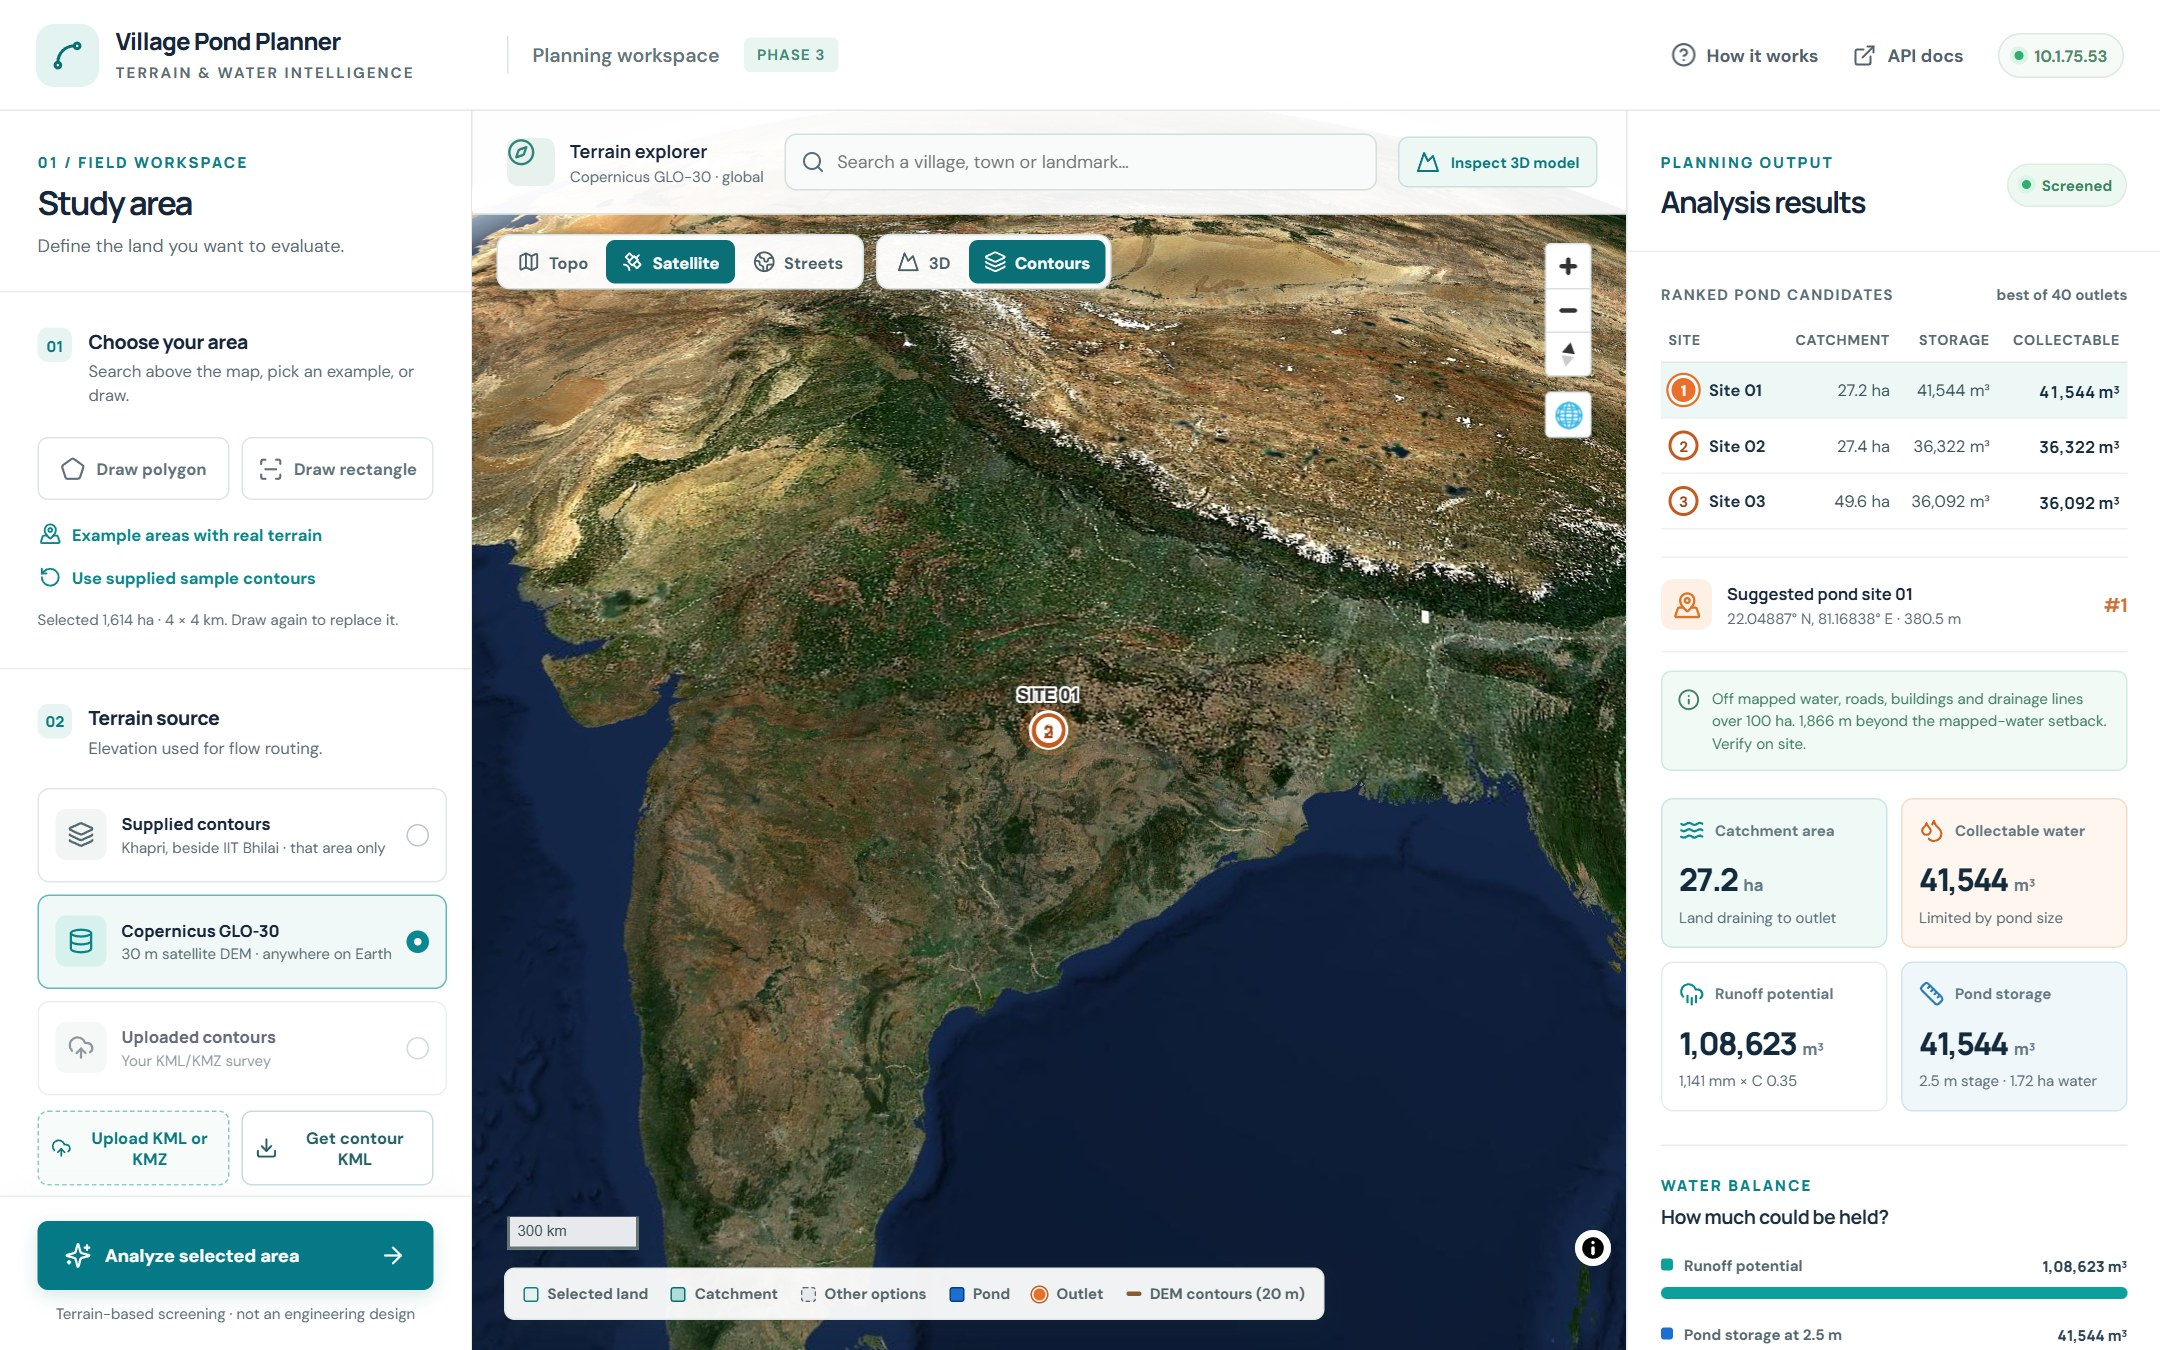
\includegraphics[width=\linewidth]{r06-globe.jpg}\caption{Globe view; the site marker sits in central India.}\end{subfigure}
\caption{The same analysis on a 2D topographic map and on the globe. The cover shows it in tilted 3D over satellite imagery.}
\label{fig:earth}
\end{figure}

\subsection{3D model of the analysis grid}
\textbf{Inspect 3D model} opens a Three.js rendering of the \emph{same} elevation grid used for routing (downsampled to at most $120\times120$), not a separate terrain service. It shows:
\begin{itemize}
\item a hypsometric colour ramp with contours draped on the surface;
\item the study-area outline, the tinted catchment, the pond surface at crest level, and numbered outlets for all three sites.
\end{itemize}
The vertical exaggeration is set automatically so that relief spans about 12\,\% of the model width (Equation~\ref{eq:exaggeration}); a slider adjusts it. \textbf{Satellite drape} textures the mesh with Sentinel-2 tiles (Figure~\ref{fig:inspector}). The exaggeration changes only the drawing, never the numbers.

\begin{figure}[htbp]
\centering
\begin{subfigure}[t]{0.49\linewidth}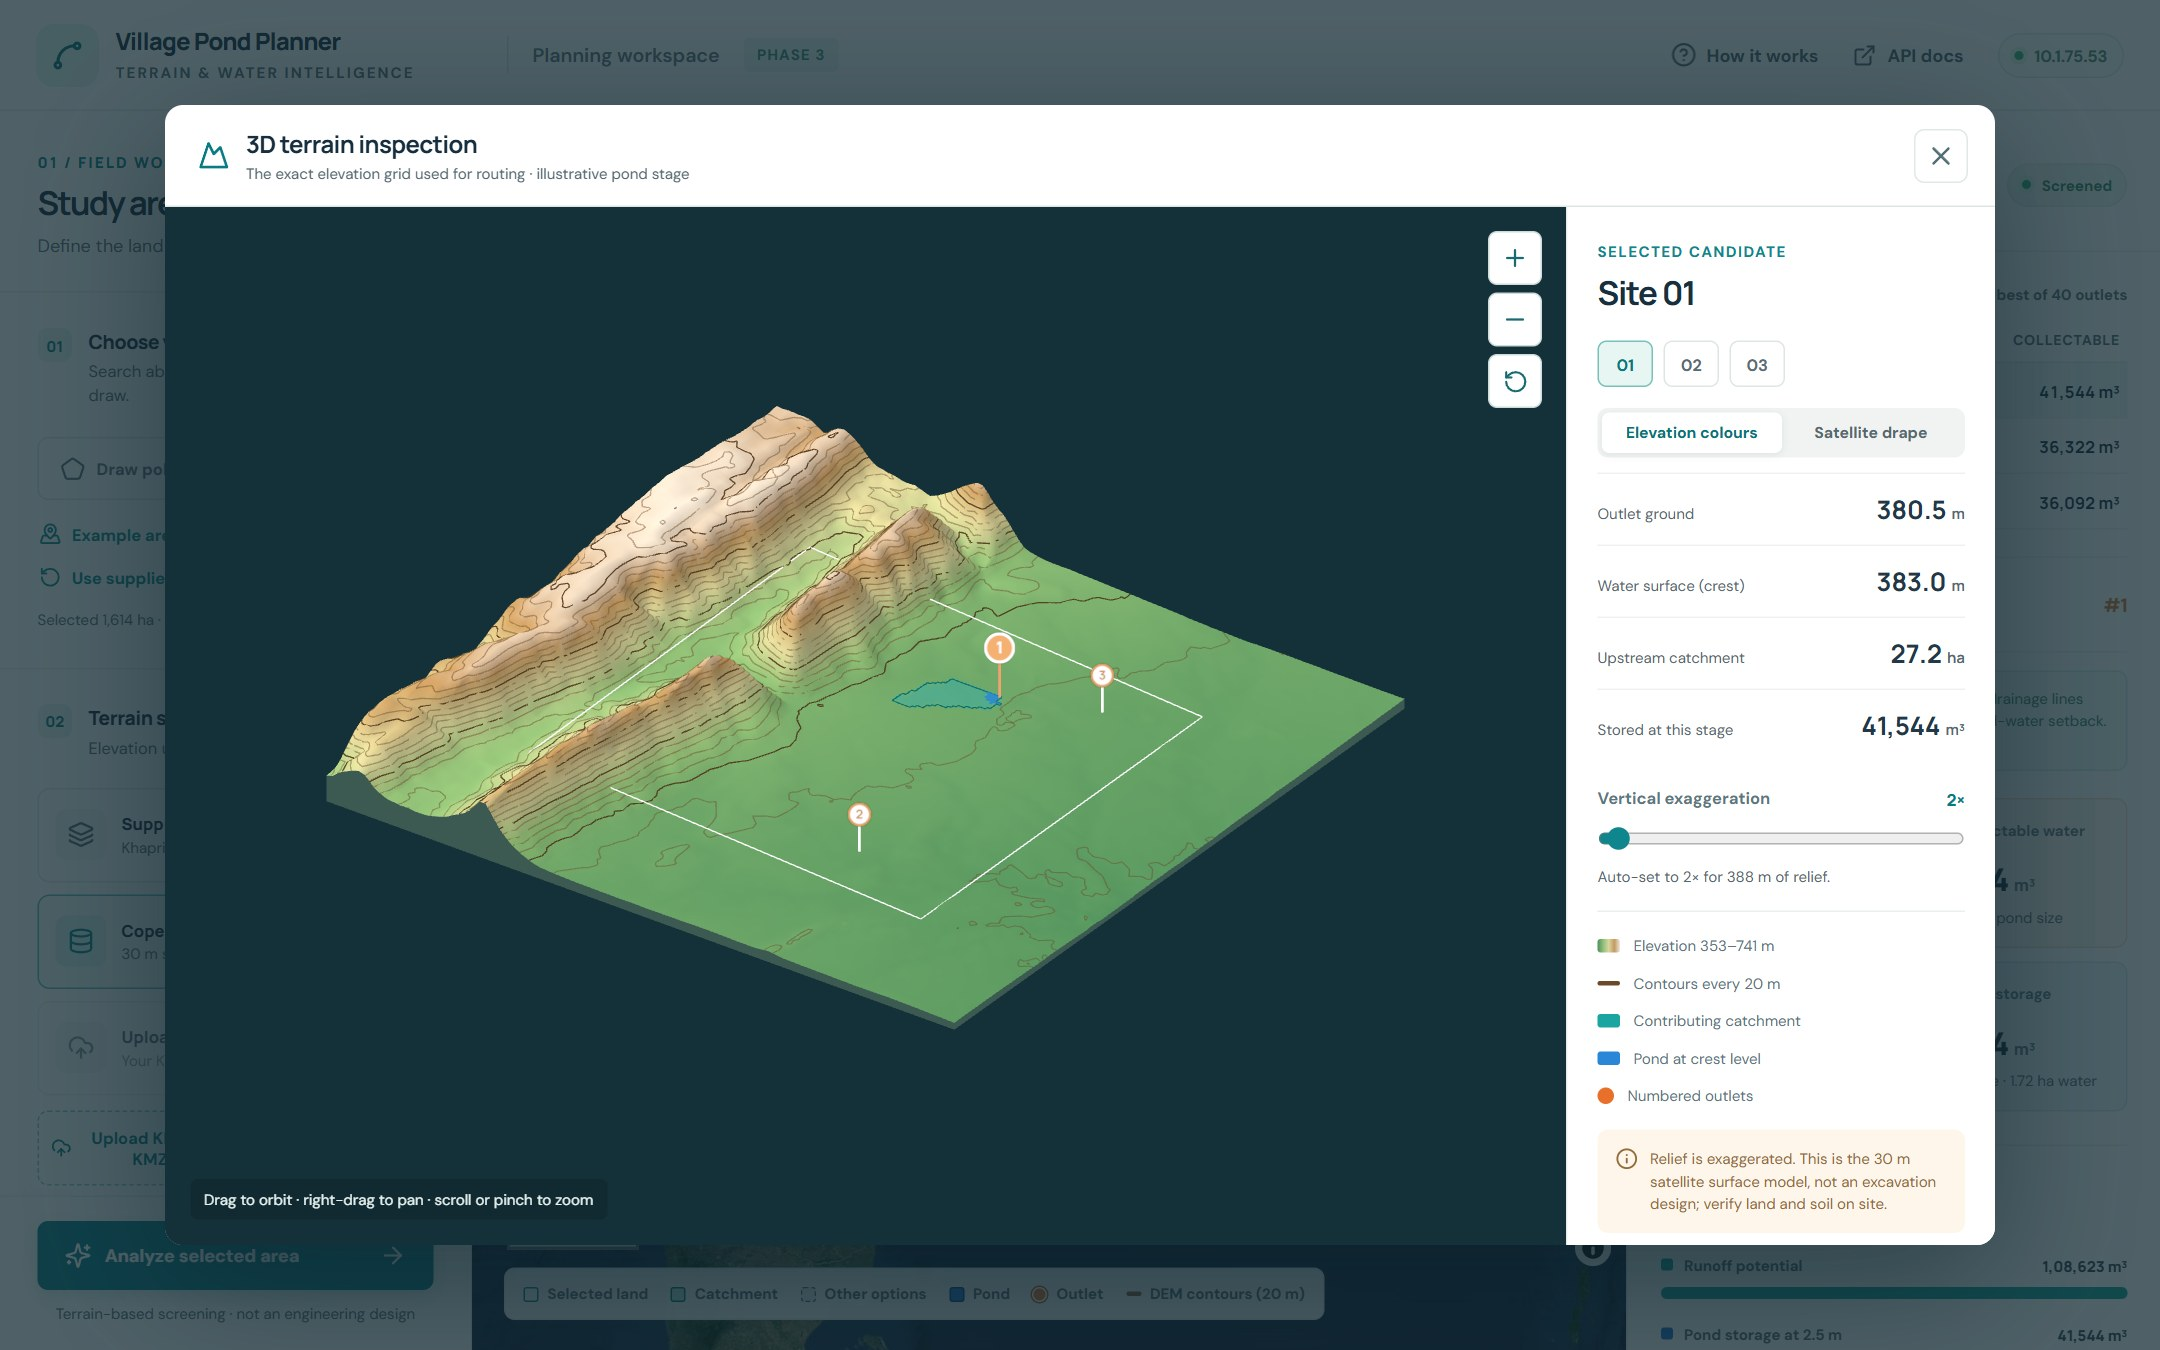
\includegraphics[width=\linewidth]{r08-inspector-relief.jpg}\caption{Elevation colours with contours and catchment.}\end{subfigure}\hfill
\begin{subfigure}[t]{0.49\linewidth}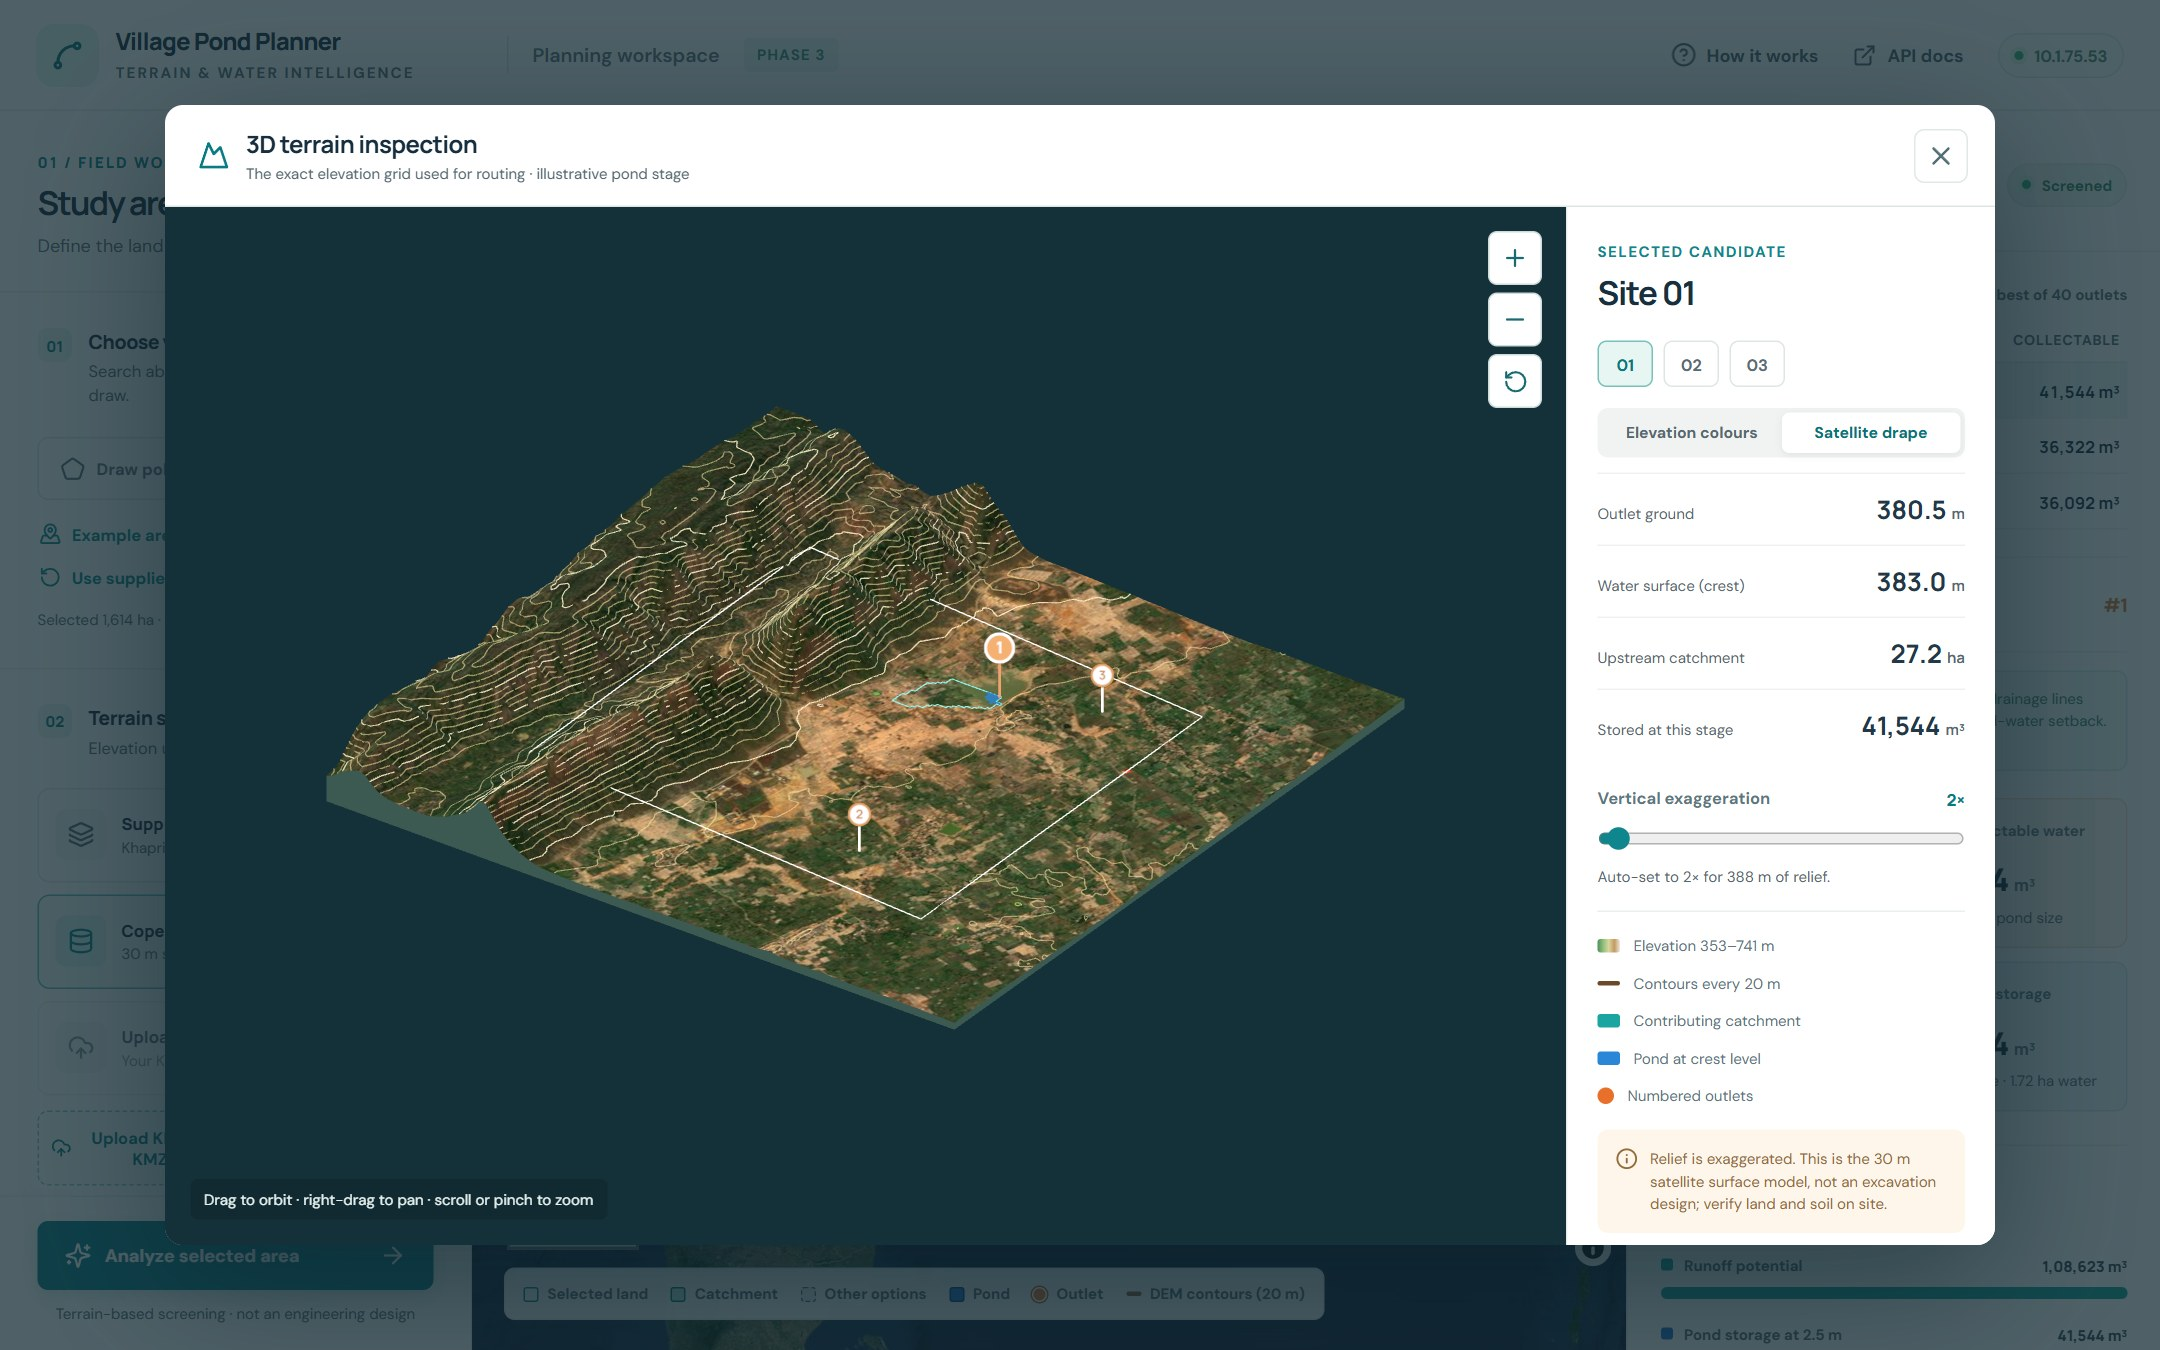
\includegraphics[width=\linewidth]{r09-inspector-imagery.jpg}\caption{Sentinel-2 satellite drape on the same mesh.}\end{subfigure}
\caption{3D inspector for the Maikal ridge front (live server).}
\label{fig:inspector}
\end{figure}

\subsection{Exports}
\begin{itemize}
\item \textbf{Google Earth KML}: the study area, three catchments, ponds and outlets, styled and clamped to terrain, with every metric in each placemark's description. It opens directly in Google Earth's 3D globe.
\item \textbf{GeoJSON}: the same features with numeric properties, for QGIS or other GIS tools.
\item \textbf{Contour KML}: real contours for the selected area at a relief-based interval, with provenance and the Copernicus attribution in the file.
\end{itemize}

\subsection{Mobile layout and accessibility}
On phones the controls slide in from the side, and the map, results and a sticky \textbf{Analyze} button stack vertically (Figure~\ref{fig:mobile}). Every grey text colour was checked against WCAG AA. About 30 colours below a 4.5:1 contrast ratio were darkened, and the minimum text size was raised. The chart palette (teal runoff, blue storage, orange collectable) passed a colour-blindness separation check. Charts have legends and table views, so colour is never the only cue. The help dialog and 3D view close with Escape.

\begin{figure}[htbp]
\centering
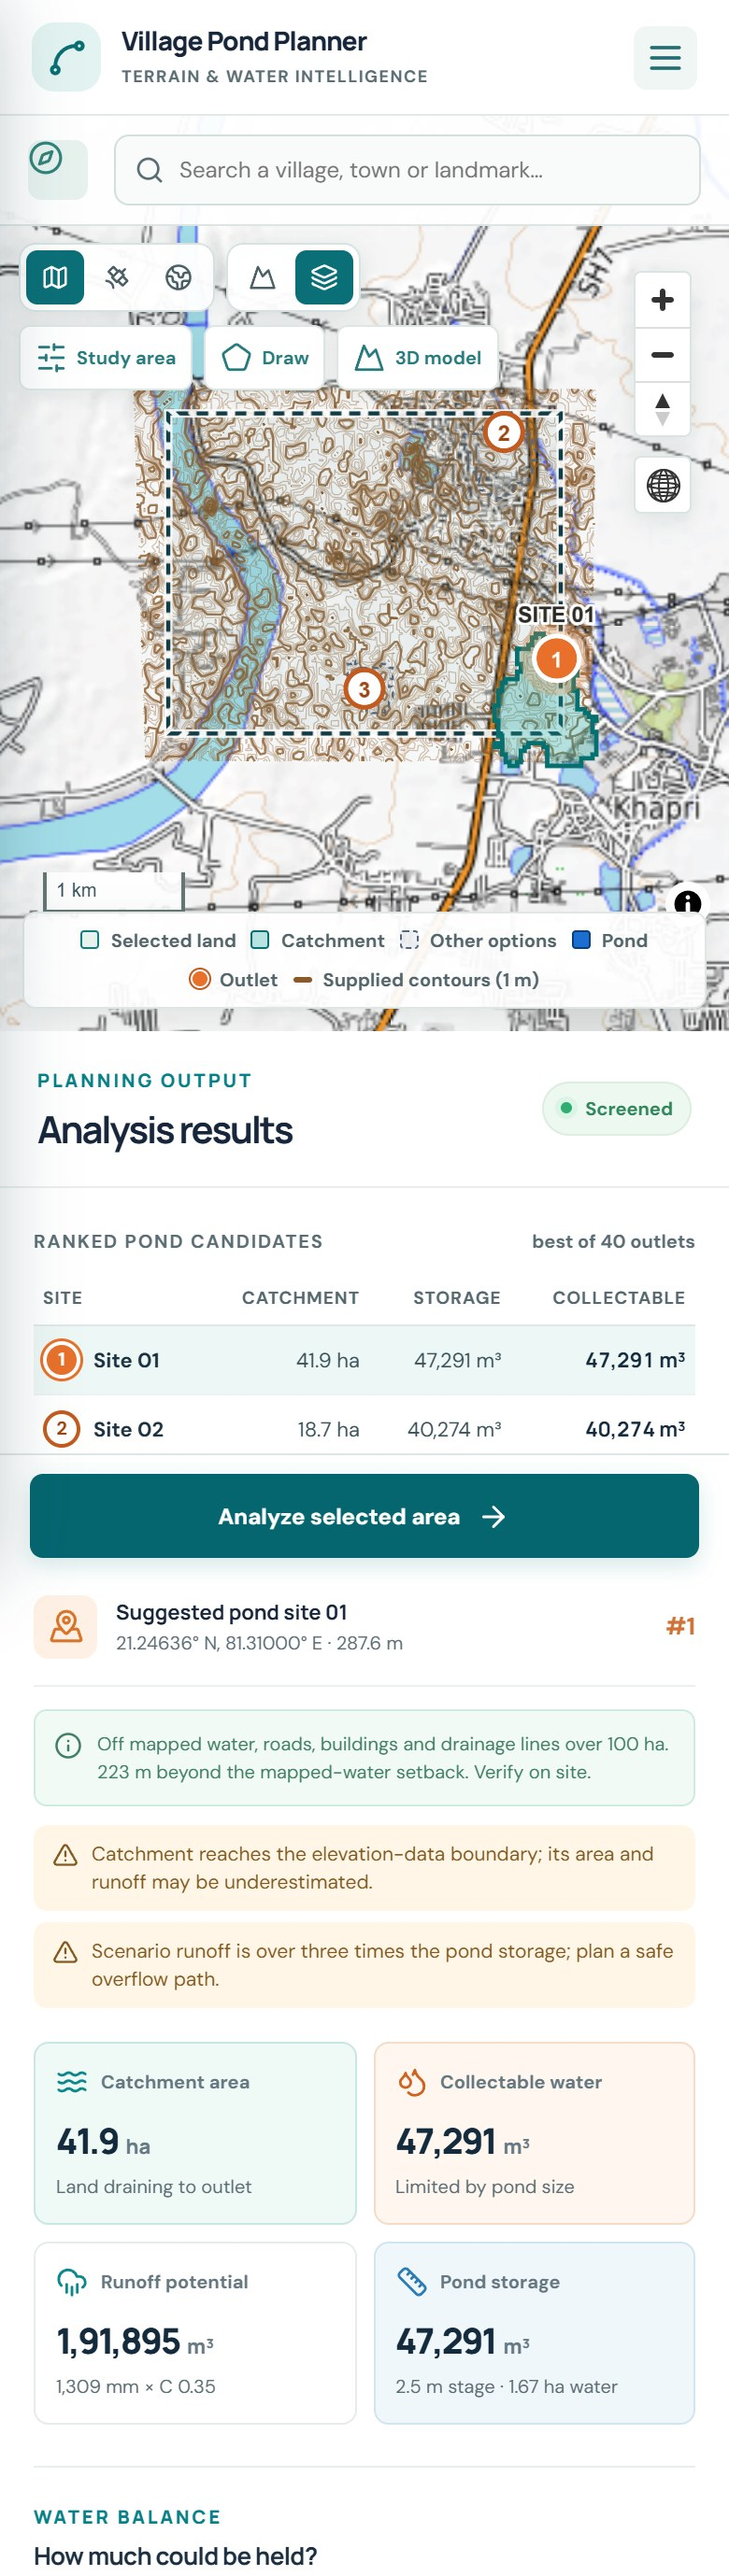
\includegraphics[width=0.3\linewidth]{r10-mobile-1.jpg}\hspace{6mm}
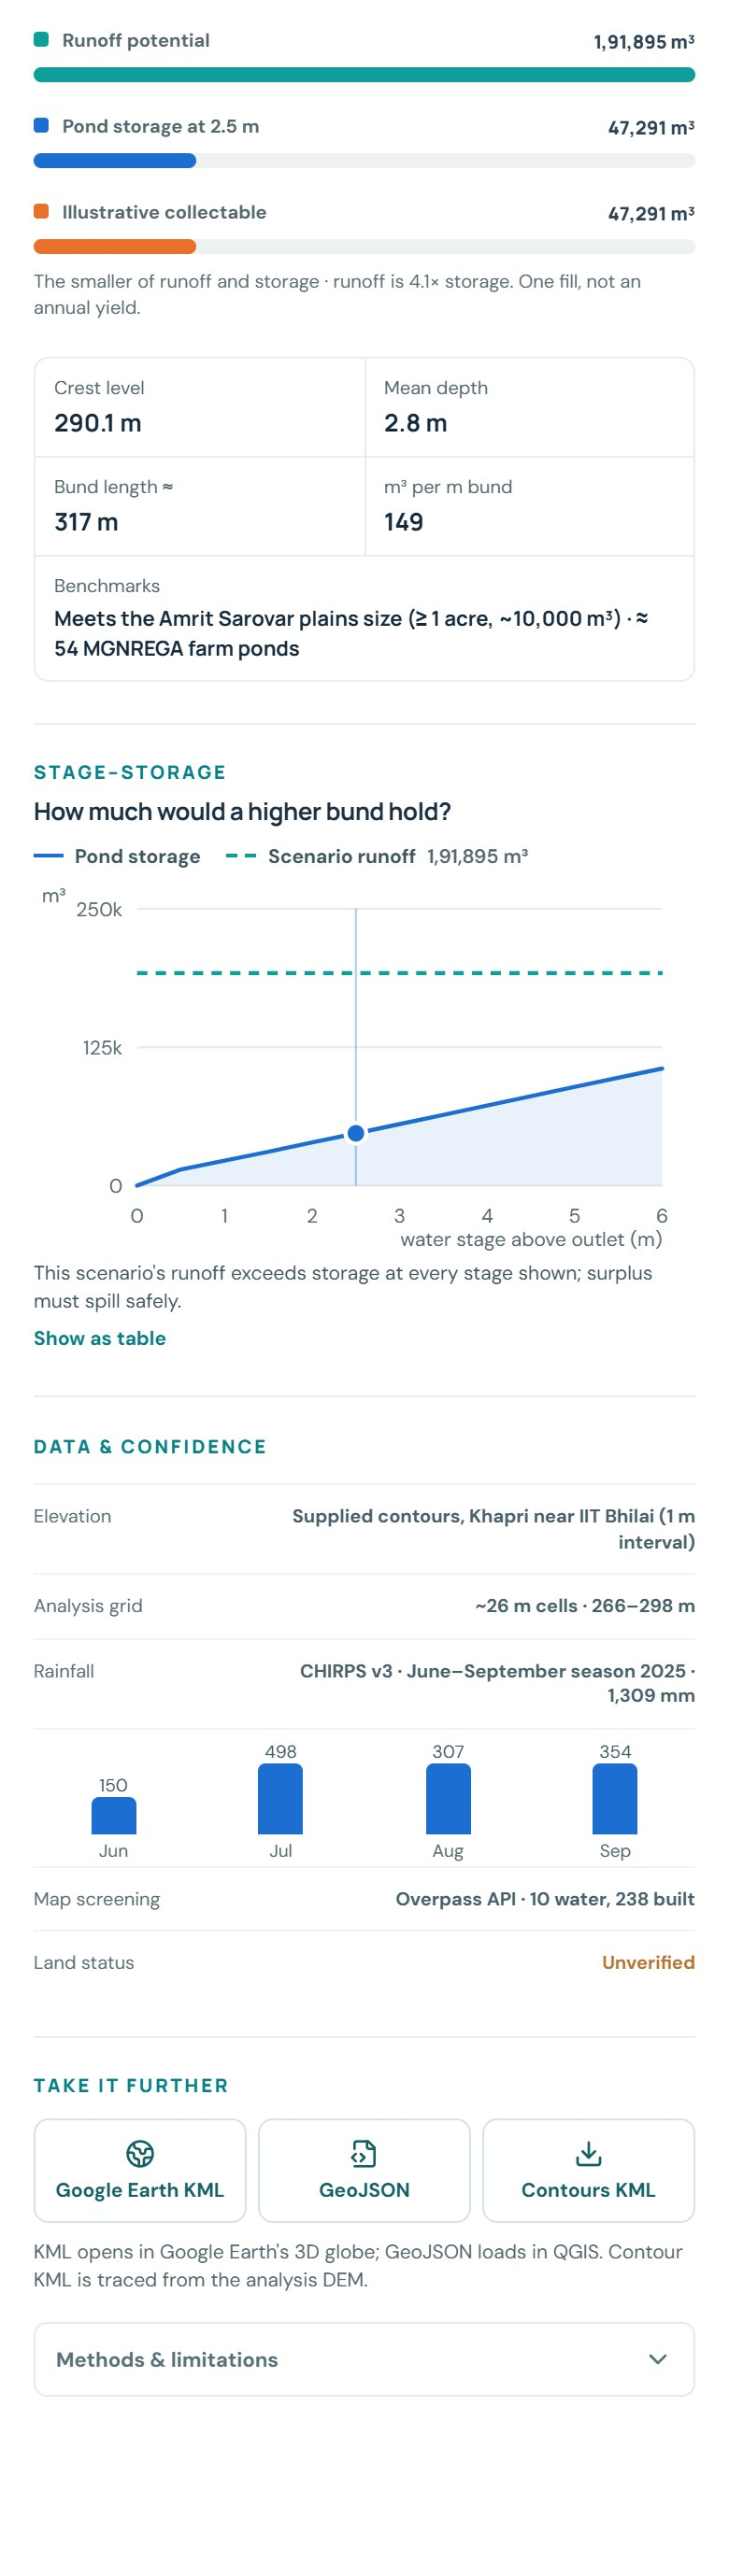
\includegraphics[width=0.3\linewidth]{r10-mobile-2.jpg}
\caption{Mobile layout (390\,px wide) on the live server, shown in two halves.}
\label{fig:mobile}
\end{figure}

% ------------------------------------------------------------------ 5
\section{Algorithms}
\label{sec:algorithms}
The analysis is deterministic. Given the same polygon, elevation source and settings it returns the same result, so results can be checked and reproduced. Algorithm version: \code{priority-flood-d8-impoundment-v4}.

\subsection{Coordinates and grids}
The polygon is validated: a simple polygon of at most 1,000 vertices, 0.25--10,000\,ha, and no wider than 20\,km. Longitude $\lambda$ and latitude $\phi$ are projected to local metres around an origin $(\lambda_0,\phi_0)$ with $R=6{,}371{,}000$\,m:
\begin{equation}
x = R\cos\phi_0\,(\lambda-\lambda_0),\qquad y = R\,(\phi-\phi_0),\qquad A_{\mathrm{cell}} = |\Delta x\,\Delta y|.
\end{equation}

\paragraph{Contour sources.} Contour vertices are interpolated to a regular grid of up to 220 cells along the longer side (the sample uses 125). A linear (triangulated) surface is flat wherever all three vertices of a triangle lie on one contour, which happens on hilltops and valley floors. With 20\,m contours, 22.5\,\% of cells were flat, and a ``pond'' there became a flat patch whose storage was simply footprint $\times$ stage. Phase~3 therefore uses a $C^1$ Clough--Tocher surface $z_{\mathrm{CT}}$, bounded by the contour interval $\Delta$:
\begin{equation}
\tilde z = \operatorname{clip}\bigl(z_{\mathrm{CT}},\; z_{\mathrm{lin}}-\Delta,\; z_{\mathrm{lin}}+\Delta\bigr).
\end{equation}
Between two drawn contours the ground cannot cross another contour level, so this bound keeps the smooth surface consistent with the survey. It removes the overshoot that unbounded cubic interpolation produces (318\,m on a survey whose top contour is 298\,m). Outside the linework's convex hull the nearest value is used. The Phase~2 route keeps linear interpolation, so its published results stay reproducible.

\paragraph{Copernicus source.} The selected area's bounding box is buffered by 30\,\% of its span, and by at least 0.009\textdegree{} ($\approx$1\,km). The 1\textdegree{} GLO-30 Cloud-Optimized GeoTIFFs that cover it are read from AWS Open Data and resampled bilinearly to at most $280\times280$ cells ($\approx$30\,m). Any gap is filled from Microsoft Planetary Computer's copy. A box that crosses tile seams was tested and has no gaps.

\subsection{Depression filling, D8 routing and accumulation}
Depressions are filled with a priority flood from the grid edge. Cells are visited in order of spill elevation, and each unvisited neighbour $n$ of the current cell $c$ is raised to at least $z'_c+\varepsilon$ ($\varepsilon=10^{-5}$\,m). Flats therefore drain without cycles:
\begin{equation}
z'_n = \max\left(z_n,\; z'_c + \varepsilon\right).
\end{equation}
Each cell $i$ drains to the neighbour $n\in N_8(i)$ with the steepest downhill grade, where $d(i,n)$ is the orthogonal or diagonal distance:
\begin{equation}
f(i) = \underset{n\in N_8(i),\;z'_n<z'_i}{\operatorname{arg\,max}}\;\frac{z'_i-z'_n}{d(i,n)}.
\end{equation}
Contributing area accumulates along this graph in topological order:
\begin{equation}
A(i) = A_{\mathrm{cell}} + \sum_{k:\,f(k)=i} A(k),\qquad C(o)=\{\,i : \text{the flow path from } i \text{ reaches } o\,\}.
\end{equation}

\subsection{Screening}
OpenStreetMap features for the area (plus a margin of about 200\,m) are read from the Overpass API and turned into exclusion masks (Table~\ref{tab:buffers}). Each exclusion is inflated by half a cell diagonal, so that no retained cell footprint crosses a mapped boundary. A partial or timed-out Overpass answer is treated as a failure, because it could silently miss water; the result is then labelled \emph{unverified}. Drainage lines with more than $A_{\max}$ of upstream area (default 100\,ha), and their neighbours, are not used as small-pond outlets: a pond there would need an engineered spillway.

\begin{table}[htbp]
\centering\small
\begin{tabular}{@{}ll@{}}
\toprule
\textbf{Mapped feature (OSM tags)} & \textbf{Exclusion buffer}\\
\midrule
Water bodies, wetlands, reservoirs, basins, \code{water=*} & 40\,m setback\\
Rivers and canals / streams, ditches and drains & 45\,m / 25\,m\\
Buildings and built-up land use (residential, commercial, industrial, retail, military, cemetery) & 12\,m\\
Motorway, trunk / primary / secondary / tertiary & 35 / 30 / 25 / 18\,m\\
Unclassified, residential, road / service, living street & 12 / 8\,m\\
Tracks, paths, footways and other minor ways / railways & 4 / 30\,m\\
\bottomrule
\end{tabular}
\caption{Approximate setbacks. They are screening margins, not legal setbacks. The prototype used a flat 35\,m for every road, including footpaths, which removed large amounts of village land.}
\label{tab:buffers}
\end{table}

\subsection{Candidate outlets and the impoundment model}
Candidate outlets are cells that:
\begin{itemize}
\item lie inside the selected land, off the exclusions and at least two cells from the grid edge;
\item drain between $\max(1\,\text{ha}, 5A_{\mathrm{cell}})$ and $A_{\max}$.
\end{itemize}
Taken in order of contributing area, up to 40 are kept, each at least $\max(200\,\text{m}, 3\text{ cells})$ apart.

For an outlet $o$ at ground elevation $z_o$ and water stage $h$, an embankment would hold water up to the crest $h_c = z_o + h$. The flooded set $P$ contains every cell $j$ that is connected to $o$ by 4-neighbour steps within $P$ and satisfies all of:
\begin{equation}
j\in C(o),\qquad z_j \le h_c,\qquad j\ \text{allowed},\qquad \lVert \mathbf{x}_j-\mathbf{x}_o\rVert \le r,
\end{equation}
where $r = \max(100\,\text{m}, 4\text{ cells})$ keeps the pond at village scale. Storage, footprint and indicative embankment length are then
\begin{equation}
V_S = \sum_{j\in P}(h_c - z_j)\,A_{\mathrm{cell}},\qquad A_P = |P|\,A_{\mathrm{cell}},\qquad
L_E = \sum_{\substack{(j,k):\, j\in P,\ k\notin C(o)\\ z_k\le h_c}} \ell_{jk},
\end{equation}
where $\ell_{jk}$ is the length of the shared cell edge. Lower ground \emph{outside} the catchment is where water would escape, so its edge length is the bund that has to be built. Repeating the calculation for $h = 0.5,1,\dots,6$\,m gives the stage--storage table. The Phase~3 prototype flooded every connected low cell, including cells downstream of the outlet that a pond cannot hold. Section~\ref{sec:review} shows the effect.

\subsection{Rainfall, water volume and ranking}
With rainfall depth $P_{\mathrm{mm}}$ (CHIRPS at the area centroid, or manual), catchment area $A_C$ and runoff coefficient $C$:
\begin{equation}
V_R = \frac{P_{\mathrm{mm}}}{1000}\,A_C\,C,\qquad V_c = \min(V_R, V_S),\qquad F = V_R / V_S.
\end{equation}
$V_c$ is the illustrative collectable volume for one fill, and $F$ is the fill ratio. The 40 candidates are sorted by the key
\[
\bigl(V_c\downarrow,\; V_S/L_E\downarrow,\; A_C\downarrow\bigr).
\]
Three sites are then chosen so that their ponds never overlap and, where possible, no two share more than 60\,\% of their catchments; this rule was added when two top sites turned out to be on the same drainage line. The three sites are alternatives, so their runoff is not added together.

\subsection{Contours and 3D display}
Contours are traced from the analysis grid by marching squares (contourpy) and simplified to a quarter of a cell. The interval is the smallest ``nice'' value at or above one twenty-fifth of the relief:
\begin{equation}
\Delta_c = \min\{v \in \{0.5,1,2,2.5,5,10,20,25,50,100,200\} : v \ge (z_{\max}-z_{\min})/25\}.
\end{equation}
Every fifth line is marked as major. For a model of width $S$ and relief $Z$, the 3D exaggeration is
\begin{equation}
e = \operatorname{clamp}\bigl(\operatorname{round}(0.12\,S/Z),\,1,\,30\bigr).
\label{eq:exaggeration}
\end{equation}
This replaces the prototype's fixed 15$\times$, which made flat plains look like spikes.

\subsection{Pseudocode}
\begin{lstlisting}
validate polygon (area, span, vertices)
grid <- supplied/uploaded contours (bounded smooth interpolation)  or  Copernicus GLO-30 (AWS, PC fallback, cached)
in parallel: OSM exclusions (Overpass, retried, cached);  CHIRPS totals for the chosen months (retried, cached)
z' <- priority_flood(grid.z);  f <- steepest_D8(z');  A <- accumulate(f)
allowed <- inside polygon AND NOT (mapped water OR built land)
outlets <- separated cells with 1 ha <= A <= A_max, allowed, not beside a major channel   (<= 40)
for each outlet o:
    C(o) <- upstream cells;  P <- flood_fill(o, crest = z_o + h, within C(o), allowed, radius r)
    V_S, A_P, L_E, stage table;  V_R = P_mm/1000 * A_C * C;  V_c = min(V_R, V_S)
rank by (V_c, V_S/L_E, A_C);  pick 3 with non-overlapping ponds and distinct catchments
return sites, GeoJSON geometries, contours, 3D preview, rainfall, screening status and limitations
\end{lstlisting}

\subsection{Parameters}
\begin{tabularx}{\linewidth}{@{}L{58mm}L{34mm}Y@{}}
\toprule
\textbf{Parameter} & \textbf{Default} & \textbf{Where it is set}\\
\midrule
Water stage $h$ & 2.5\,m (0.5--8) & slider, \code{stage\_m}\\
Runoff coefficient $C$ & 0.35 (0--1] & presets and slider, \code{runoff\_coefficient}\\
Small-pond catchment cap $A_{\max}$ & 100\,ha (5--5,000) & advanced slider, \code{max\_catchment\_ha}\\
Rainfall & CHIRPS Jun--Sep 2025 & \code{rainfall\_period}, \code{rainfall\_year}\\
Pond search radius $r$ & $\max(100\text{ m},4\text{ cells})$ & fixed\\
Minimum catchment & $\max(1\text{ ha},5\text{ cells})$ & fixed\\
Outlet separation / candidates & $\max(200\text{ m},3\text{ cells})$ / 40 & fixed\\
Copernicus buffer / grid & 30\,\% ($\geq$1\,km) / $\leq280^2$ cells & fixed\\
\bottomrule
\end{tabularx}

% ------------------------------------------------------------------ 6
\section{Data sources, provenance and licences}
\label{sec:data}
\begin{tabularx}{\linewidth}{@{}L{38mm}L{34mm}Y@{}}
\toprule
\textbf{Source} & \textbf{Used for} & \textbf{Licence and attribution}\\
\midrule
Copernicus DEM GLO-30 via AWS Open Data~[\ref{ref:glo30}] (fallback: Planetary Computer) & Analysis elevation (surface model, EGM2008 heights), contour export & \copyright{} DLR e.V. 2010--2014 and \copyright{} Airbus Defence and Space GmbH 2014--2018, provided under COPERNICUS by the EU and ESA\\
CHIRPS v3 monthly~[\ref{ref:chirps}] & Rainfall & CC BY 4.0; doi:10.15780/G2JQ0P\\
OpenStreetMap via Overpass~[\ref{ref:overpass}] & Water and built-land screening & ODbL, \copyright{} OpenStreetMap contributors\\
OpenTopoMap & Topographic basemap & CC-BY-SA\\
EOxCloudless 2025~[\ref{ref:eox}] & Satellite basemap and 3D drape & CC BY-NC-SA 4.0: non-commercial academic use\\
OpenStreetMap tiles & Street basemap & OSMF tile usage policy\\
Terrain Tiles on AWS & MapLibre 3D terrain only & SRTM and GMTED2010 courtesy of USGS; ETOPO1 courtesy of NOAA\\
Photon (komoot) & Place search & OSM data; public server used within fair use\\
\bottomrule
\end{tabularx}

Two sources were deliberately rejected after checking their terms:
\begin{itemize}
\item \textbf{Esri World Imagery} requires an ArcGIS account for this kind of use.
\item \textbf{The OpenStreetMap editing API}, which the prototype used, is reserved for editing, not read-only applications. It also refused a 14$\times$12\,km area.
\end{itemize}

\begin{warnbox}[title=Provenance of the supplied contour map]
\code{contours\_1m.kml} covers 81.281--81.313\textdegree E, 21.240--21.264\textdegree N. That is Khapri village farmland between the IIT Bhilai campus (centre about 81.318\textdegree E, 21.245\textdegree N) and the Shivnath river, and only a thin strip overlaps the campus. Its internal structure (a root \code{Folder} named \code{ContourMapGenerator} and lxml \code{py:pytype} attributes) matches exports from the free Contour Map Generator~[\ref{ref:cmg}], which traces roughly 30\,m satellite elevation. The 1\,m contour interval is therefore finer than the real precision of the data. The planner labels it as supplied contours, not a field survey, and says so in its limitations.
\end{warnbox}

Better sources for detailed design include:
\begin{itemize}
\item \textbf{Survey of India Open Series Maps}: free 1:50,000 GeoPDFs with 20\,m contours, which need digitising~[\ref{ref:soi}];
\item \textbf{ISRO Bhuvan CartoDEM v3}: 30\,m, login required;
\item \textbf{FABDEM}: bare-earth 30\,m, non-commercial;
\item \textbf{a village DGPS or drone survey} exported as contour KML.
\end{itemize}
Any DEM can be converted with \code{gdal\_contour -f KML -i 5 -a elevation dem.tif out.kml}, and the planner reads the \code{elevation} attribute.

% ------------------------------------------------------------------ 7
\section{Verified example areas}
\label{sec:examples}
Each area was run end to end with the final algorithm: GLO-30 elevation, the CHIRPS June--September 2025 total, Overpass screening, three ranked sites and contour export. Its contours are shipped in \code{contour-maps/real/}. The areas were chosen for real hill-to-plain relief with villages and seasonal drainage. The Ralegan Siddhi, Hiware Bazar, Alwar, Sukhomajri and Abreha we Atsbeha areas are known for community watershed work.

\begin{table}[htbp]
\centering\small
\begin{tabularx}{\linewidth}{@{}L{44mm}Yrrrr@{}}
\toprule
\textbf{Area} & \textbf{Region} & \textbf{Relief (m)} & \textbf{Monsoon (mm)} & \textbf{Site 1 (ha)} & \textbf{Site 1 (\mthree)}\\
\midrule
Khapri (supplied contours) & Durg, beside IIT Bhilai & 266--298 & 1,309 & 41.9 & 47,291\\
Dongargarh--Khairagarh ridge & $\sim$48\,km W & 338--632 & 1,337 & 34.0 & 44,051\\
Maikal ridge front & Kabirdham, $\sim$90\,km N & 353--741 & 1,141 & 27.2 & 41,544\\
Kanker west & $\sim$110\,km S & 392--682 & 1,287 & 31.1 & 53,625\\
Sihawa, Mahanadi source & Dhamtari, $\sim$120\,km SE & 426--550 & 1,287 & 56.4 & 43,319\\
Mainpat plateau & Surguja, $\sim$265\,km NE & 1,026--1,120 & 1,626 & 21.3 & 15,196\\
Ralegan Siddhi & Maharashtra & 611--747 & 623 & 25.8 & 24,315\\
Hiware Bazar & Maharashtra & 684--876 & 665 & 97.0 & 32,525\\
Bheekampura johads & Alwar, Rajasthan & 393--634 & 1,130 & 17.2 & 39,658\\
Sukhomajri & Panchkula, Haryana & 426--606 & 1,538 & 26.4 & 23,998\\
Abreha we Atsbeha & Tigray, Ethiopia & 1,926--2,539 & 681 & 54.2 & 26,191\\
\bottomrule
\end{tabularx}
\caption{Example areas (June--September 2025 CHIRPS, $C=0.35$, 2.5\,m stage). Site 1 is the best-ranked outlet; in every area it is limited by storage, not runoff. The Khapri row uses the supplied contours, so its relief is the grid's, not GLO-30's.}
\label{tab:examples}
\end{table}

\begin{figure}[htbp]
\centering
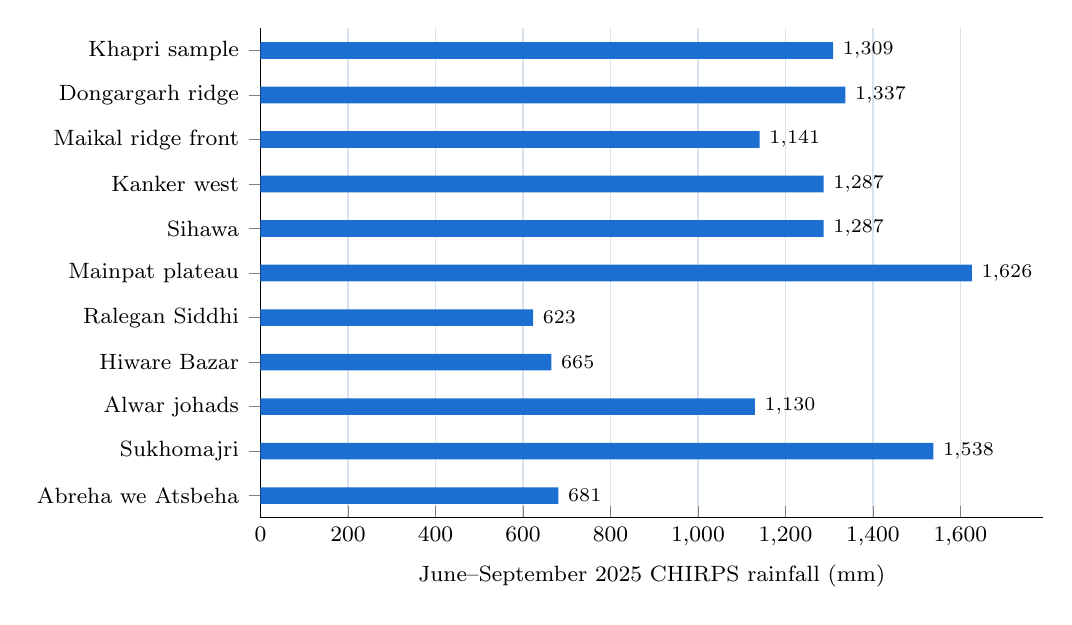
\begin{tikzpicture}
\begin{axis}[xbar, width=0.95\linewidth, height=78mm, bar width=6pt, xmin=0,
  symbolic y coords={Abreha we Atsbeha,Sukhomajri,Alwar johads,Hiware Bazar,Ralegan Siddhi,Mainpat plateau,Sihawa,Kanker west,Maikal ridge front,Dongargarh ridge,Khapri sample},
  ytick=data, y tick label style={font=\footnotesize}, x tick label style={font=\footnotesize,/pgf/number format/1000 sep={\mathord{,}}},
  xlabel={June--September 2025 CHIRPS rainfall (mm)}, xlabel style={font=\footnotesize},
  nodes near coords, nodes near coords style={font=\scriptsize,/pgf/number format/1000 sep={\mathord{,}}}, enlarge y limits=0.05,
  axis lines*=left, xmajorgrids, grid style={line}]
\addplot[fill=storage,draw=none] coordinates {(681,Abreha we Atsbeha) (1538,Sukhomajri) (1130,Alwar johads) (665,Hiware Bazar) (623,Ralegan Siddhi) (1626,Mainpat plateau) (1287,Sihawa) (1287,Kanker west) (1141,Maikal ridge front) (1337,Dongargarh ridge) (1309,Khapri sample)};
\end{axis}
\end{tikzpicture}
\caption{Monsoon rainfall read from CHIRPS for each example. The drought-prone Maharashtra villages receive half the rainfall of the Chhattisgarh sites. For comparison, the IMD 1991--2020 normal for Raipur is about 1,145\,mm for June--September.}
\end{figure}

For Kanker west the stage--storage curve shows how a higher bund trades embankment length for water (Figure~\ref{fig:stage}). At the default 2.5\,m stage the pond holds 53,625\,\mthree{}. The season's runoff of about 140,000\,\mthree{} would fill it to about 6\,m. That exceeds the Mission Amrit Sarovar plains benchmark (at least 1 acre and about 10,000\,\mthree{}) and equals about 61 MGNREGA model farm ponds.

\begin{figure}[htbp]
\centering
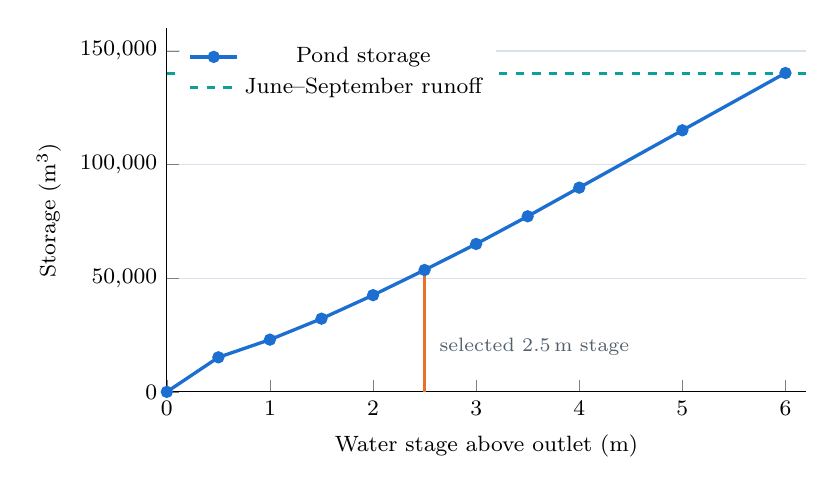
\begin{tikzpicture}
\begin{axis}[width=0.8\linewidth,height=62mm,xmin=0,xmax=6.2,ymin=0,ymax=160000,
  xlabel={Water stage above outlet (m)},ylabel={Storage (\mthree)},
  y tick label style={/pgf/number format/1000 sep={\mathord{,}},font=\footnotesize},x tick label style={font=\footnotesize},
  label style={font=\footnotesize},scaled y ticks=false,ymajorgrids,grid style={line},axis lines*=left,
  legend style={font=\footnotesize,draw=none,at={(0.02,0.98)},anchor=north west}]
\addplot[storage,very thick,mark=*,mark size=1.6pt] coordinates {(0,0) (0.5,15205) (1,22982) (1.5,32205) (2,42559) (2.5,53625) (3,65076) (3.5,77255) (4,89864) (5,115082) (6,140301)};
\addlegendentry{Pond storage}
\addplot[runoff,very thick,dashed,domain=0:6.2] {140002};
\addlegendentry{June--September runoff}
\draw[collect,thick] (axis cs:2.5,0) -- (axis cs:2.5,53625);
\node[font=\scriptsize,text=muted,anchor=west] at (axis cs:2.55,20000) {selected 2.5\,m stage};
\end{axis}
\end{tikzpicture}
\caption{Stage--storage curve for the best Kanker west site (live result). Storage rises with stage while the embankment grows from 30\,m to 240\,m, so the curve helps choose a bund height.}
\label{fig:stage}
\end{figure}

% ------------------------------------------------------------------ 8
\clearpage
\section{Quality review: defects found and fixed}
\label{sec:review}
The Phase~3 prototype (26 September 2026) was reviewed with probe scripts, live network tests and browser screenshots. Every defect below was reproduced before it was fixed and is now covered by a test.

\begin{tabularx}{\linewidth}{@{}L{28mm}YY@{}}
\toprule
\textbf{Area} & \textbf{Defect (measured)} & \textbf{Fix}\\
\midrule
Pond storage & Pond cells spread downstream and sideways outside the outlet's own catchment. That was 25--54\,\% of each footprint, and it inflated storage by 37--272\,\% (Figure~\ref{fig:inflation}). & Impoundment model restricted to $C(o)$; the embankment length comes from lower ground outside it.\\
Ranking & Sites were the cells just below an arbitrary 98th-percentile ``channel'' cutoff. All three had 32--36\,ha catchments on the sample (cutoff 36.3\,ha), and storage never affected the rank. & 40 separated candidates ranked by collectable volume; an explicit small-pond catchment cap.\\
Terraces & Linear interpolation of 20\,m contours left 22.5\,\% of cells flat. Two sites shared one drainage line, and their storage was footprint $\times$ stage. & Bounded Clough--Tocher surface (0.6\,\% flat) and catchment-diversity rule.\\
OSM screening & The prototype used the editing API against its policy, and a 14$\times$12\,km area returned ``unavailable''. It applied a 35\,m buffer to every footpath. & Overpass with three servers, partial answers rejected, buffers by road class. The same area now screens 249 water and 15,361 built features.\\
Rainfall & A single month (August 2025) was treated as the planning rainfall. & Monsoon and annual CHIRPS totals fetched in parallel, with monthly bars.\\
Speed & DEM, OSM and CHIRPS were fetched one after another: 12.9\,s for a Copernicus area. & Parallel fetches, a grid cache, AWS tiles: 6.3\,s cold, 0.3\,s repeat (Figure~\ref{fig:speed}).\\
Map & Switching the terrain source destroyed the map, so the drawn area vanished while the panel still said ``Area selected''. & The map is created once and its layers are updated in place.\\
3D view & A fixed 15$\times$ exaggeration made plains look like spikes, and the skirt dominated the view. & Automatic exaggeration, a thin skirt, draped contours, satellite drape.\\
Usability & The only way to reach another area was panning; drawing outside the survey just produced an error. & Search, examples, automatic source switching, a live area check.\\
Accessibility & About 30 text colours were below WCAG AA (e.g. \#99a5a9 on white $\approx$2.6:1), and some text was 8--9\,px. & Colours darkened to at least 4.5:1; minimum sizes raised.\\
Honesty & The sample was described as a campus survey, and the runoff presets had no source. & Provenance corrected; presets cite CGWB ranges.\\
\bottomrule
\end{tabularx}

\begin{figure}[htbp]
\centering
\begin{subfigure}[t]{0.49\linewidth}
\centering
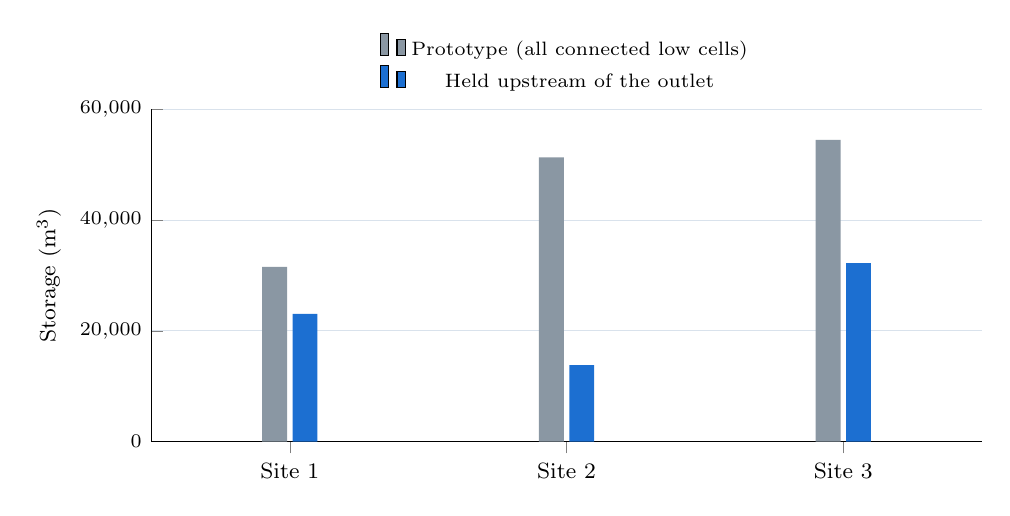
\begin{tikzpicture}
\begin{axis}[ybar,width=\linewidth,height=58mm,bar width=9pt,ymin=0,ymax=60000,
  symbolic x coords={Site 1,Site 2,Site 3},xtick=data,enlarge x limits=0.25,
  ylabel={Storage (\mthree)},label style={font=\footnotesize},scaled y ticks=false,
  y tick label style={/pgf/number format/1000 sep={\mathord{,}},font=\scriptsize},x tick label style={font=\footnotesize},
  legend style={font=\scriptsize,draw=none,at={(0.5,1.02)},anchor=south,legend columns=1},ymajorgrids,grid style={line},axis lines*=left]
\addplot[fill=old,draw=none] coordinates {(Site 1,31579) (Site 2,51368) (Site 3,54516)};
\addplot[fill=storage,draw=none] coordinates {(Site 1,23082) (Site 2,13811) (Site 3,32261)};
\legend{Prototype (all connected low cells),Held upstream of the outlet}
\end{axis}
\end{tikzpicture}
\caption{Storage inflation in the prototype (sample area).}
\label{fig:inflation}
\end{subfigure}\hfill
\begin{subfigure}[t]{0.49\linewidth}
\centering
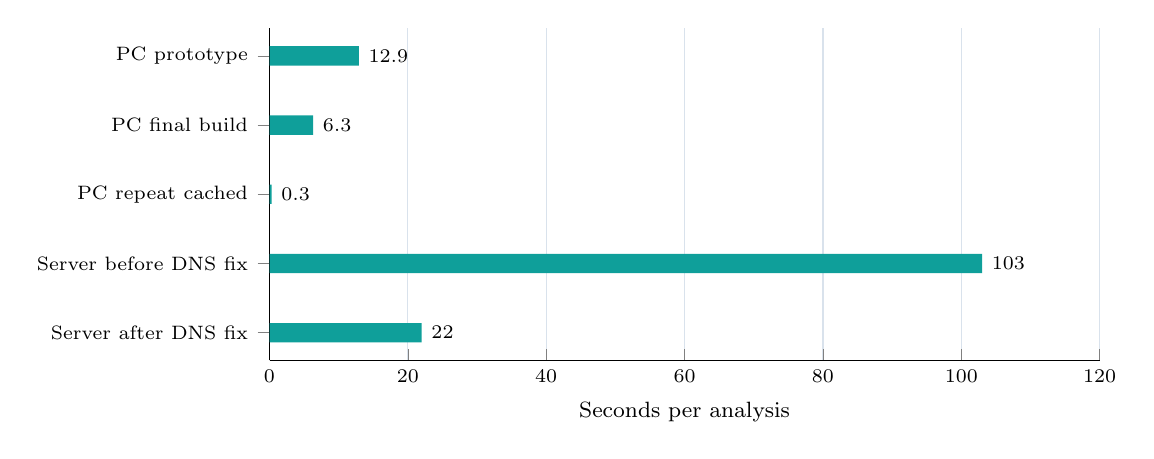
\begin{tikzpicture}
\begin{axis}[xbar,width=\linewidth,height=58mm,bar width=7pt,xmin=0,xmax=120,
  symbolic y coords={Server after DNS fix,Server before DNS fix,PC repeat cached,PC final build,PC prototype},
  ytick=data,y tick label style={font=\scriptsize},x tick label style={font=\scriptsize},
  xlabel={Seconds per analysis},label style={font=\footnotesize},nodes near coords,nodes near coords style={font=\scriptsize},
  xmajorgrids,grid style={line},axis lines*=left]
\addplot[fill=runoff,draw=none] coordinates {(12.9,PC prototype) (6.3,PC final build) (0.3,PC repeat cached) (103,Server before DNS fix) (22,Server after DNS fix)};
\end{axis}
\end{tikzpicture}
\caption{Analysis time for a Copernicus area. Server values are the worst case of the runs (69--103\,s before, 3--22\,s after).}
\label{fig:speed}
\end{subfigure}
\caption{Two of the measured improvements.}
\end{figure}

% ------------------------------------------------------------------ 9
\section{Validation}
\subsection{Automated tests}
\begin{tabularx}{\linewidth}{@{}L{36mm}rY@{}}
\toprule
\textbf{Suite} & \textbf{Tests} & \textbf{What is checked}\\
\midrule
\code{test\_api.py} & 4 & Phase 2 route: health, sample KML, KMZ, unsupported format\\
\code{test\_planning.py} & 6 & Geometries and the runoff formula; different land gives different sites; outside-area rejection; contour overlay; sites and ponds avoid mapped water and roads; OSM XML parsing\\
\code{test\_hydrology.py} & 11 & Pond inside its own catchment; ranking by collectable volume; consistent stage curves; non-overlapping ponds; higher stage holds more; contours in the response; a synthetic valley; rainfall periods; Overpass parser and road classes; contour export round trip\\
\code{test\_upload.py} & 8 & Uploaded KML/KMZ drives the analysis; absolute altitudes and ExtendedData; every shipped real KML uploads and analyzes; bounded smooth interpolation; distinct drainage lines\\
\code{test\_resilience.py} & 5 & AWS tile naming across hemispheres and seams; retries; disk cache; offline cached DEM; DNS stale-if-error\\
\bottomrule
\end{tabularx}

All 34 tests pass on the development PC and on the IIT server. Three Playwright browser suites drive a real Chrome, on desktop (1440$\times$900) and mobile (390$\times$844):
\begin{itemize}
\item \code{smoke.mjs}: analyze, draw a second area and confirm the site changes;
\item \code{smoke-upload-3d.mjs}: upload two contour maps, open the 3D model, orbit it, and change site and exaggeration;
\item \code{walkthrough.mjs}: satellite and 3D terrain, source switching, an example area, the inspector with satellite drape, the globe, and search.
\end{itemize}
Setting \code{POND\_URL=http://10.1.75.53:3233/} runs them against the live deployment, where they pass with no page errors.

\subsection{Live verification}
\begin{tabularx}{\linewidth}{@{}Yrr@{}}
\toprule
\textbf{Request on the deployed server (from the campus network)} & \textbf{HTTP} & \textbf{Time}\\
\midrule
\code{GET /}, \code{/docs}, \code{/health}, \code{/api/config}, front-end assets (JavaScript served as \code{text/javascript}) & 200 & $<$0.1\,s\\
Sample analysis with the CHIRPS monsoon total & 200 & 1.2\,s\\
Cached example areas (Maikal ridge front, Abreha we Atsbeha) & 200 & 0.7--1.1\,s\\
KML upload (106 contour lines) / contour KML export & 200 & 0.1\,s\\
Phase 2 \code{POST /analyzeContour} with the supplied KML & 200 & 2.9\,s\\
New, uncached areas (AWS DEM, CHIRPS and Overpass fetched live) & 200 & 3--22\,s\\
Cached example with \emph{all} network access blocked (proxy test) & 200 & 0.4\,s\\
\bottomrule
\end{tabularx}

% ------------------------------------------------------------------ 10
\section{Deployment on the IIT system}
\label{sec:deploy}
The application runs on the assigned container: SSH port 2233, so Application~1 is internal port 3000, published as external port 3233. It runs in tmux session \code{pond-app} under a loop script (\code{scripts/run\_server.sh}) that restarts Uvicorn if it exits and logs to \code{logs/app.log}. Figure~\ref{fig:docs} shows the live API documentation.

\begin{figure}[htbp]
\centering
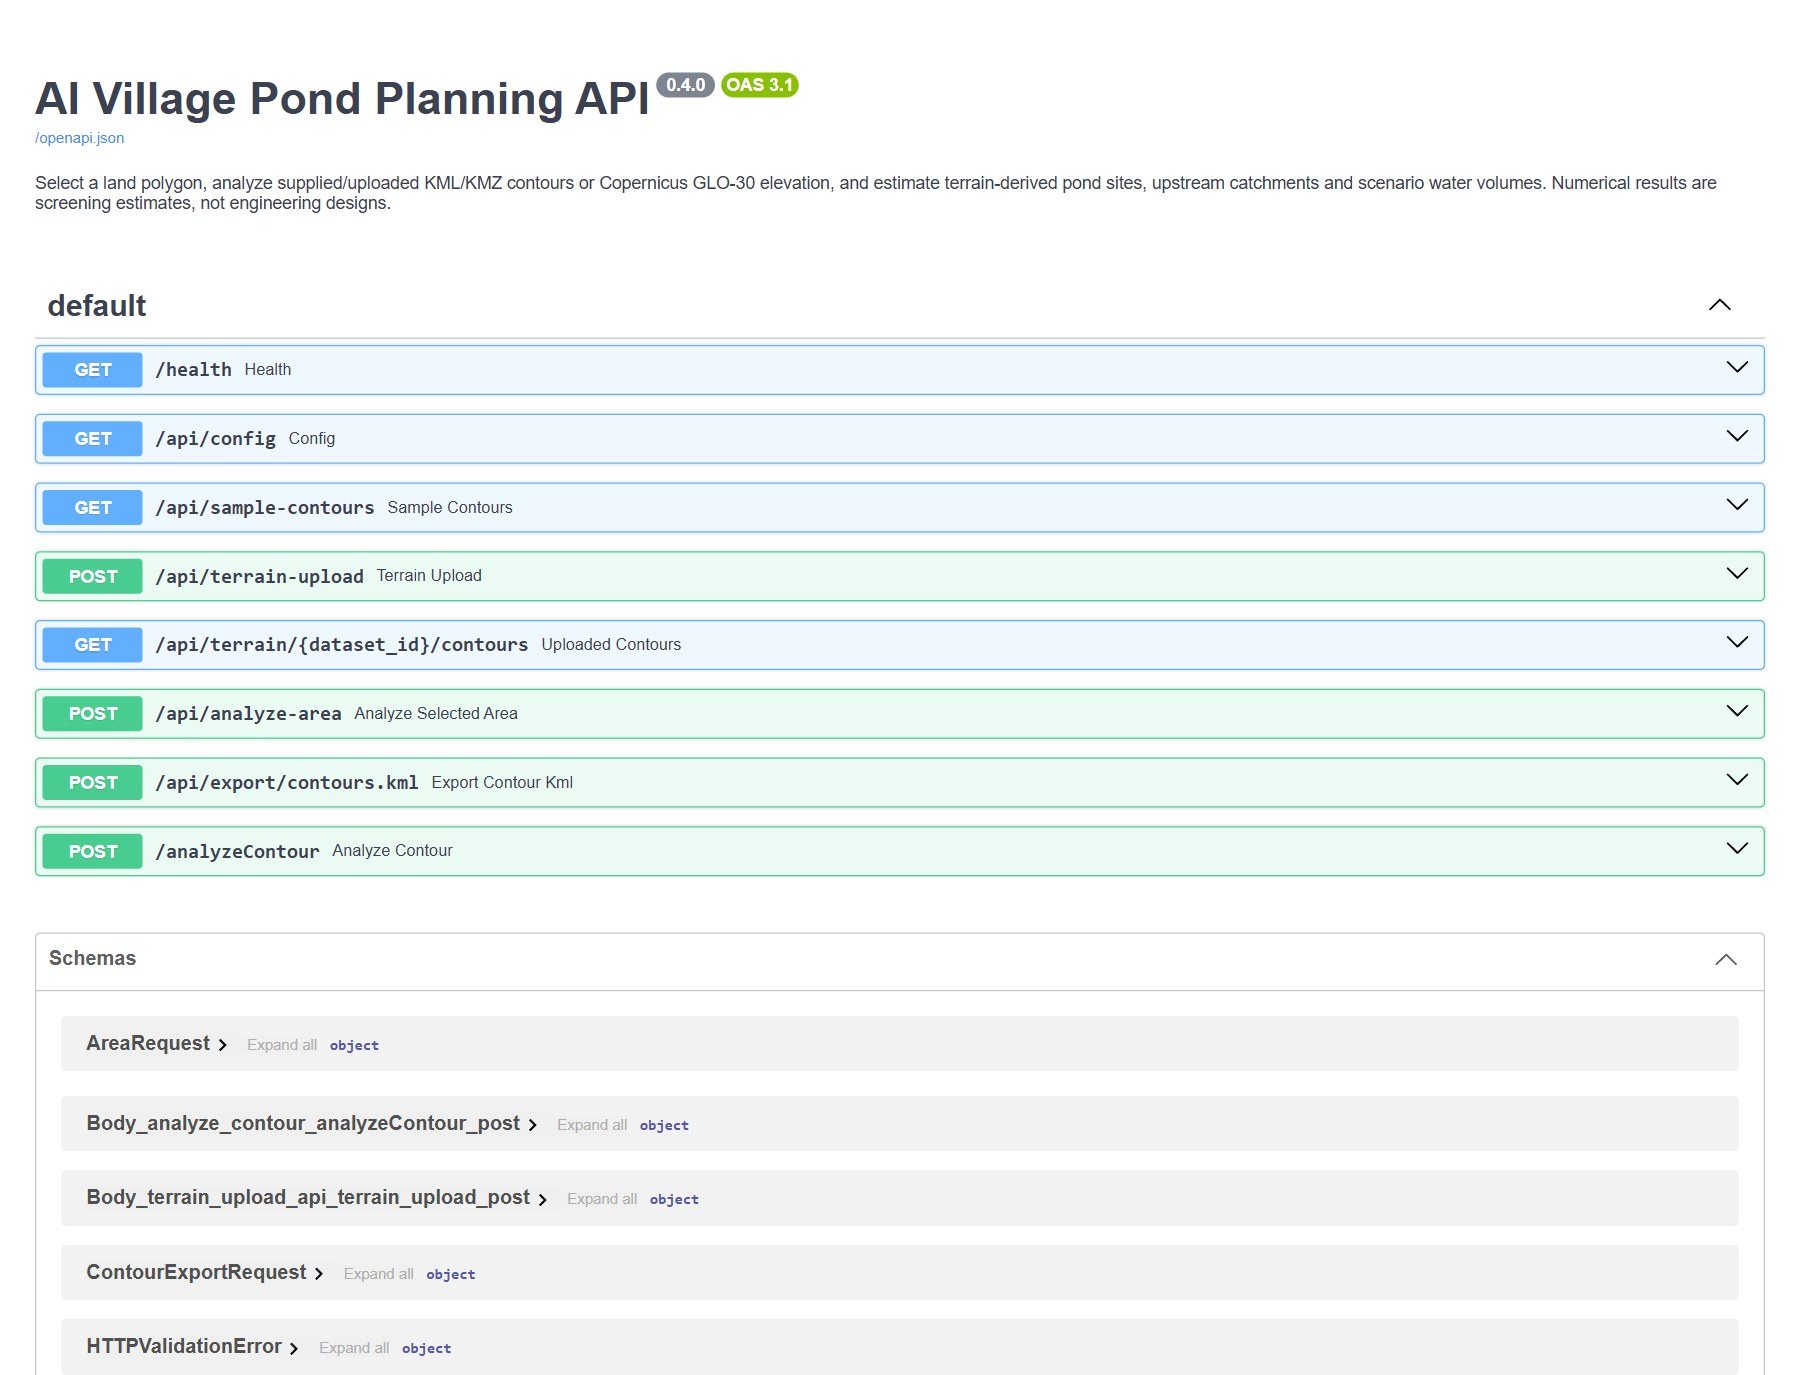
\includegraphics[width=0.78\linewidth]{r12-docs.jpg}
\caption{Swagger UI of the deployed API at \url{http://10.1.75.53:3233/docs}, listing the eight routes.}
\label{fig:docs}
\end{figure}

\subsection{Constraints found and how they were handled}
\begin{tabularx}{\linewidth}{@{}L{42mm}Y@{}}
\toprule
\textbf{Constraint (measured)} & \textbf{Handling}\\
\midrule
No Node.js; PyPI downloads failed DNS or TLS checks & The front end is built on a workstation. Linux wheels (73 packages, 101\,MB) are installed offline with \code{pip -{}-no-index}. \code{uvloop} is added explicitly, because pip on Windows skips Linux-only dependencies.\\
SFTP restricted & Files are streamed through the SSH channel and verified by SHA-256.\\
Windows line endings broke the start script & \code{.gitattributes} keeps \code{*.sh} as LF.\\
Container DNS (1.1.1.1/8.8.8.8) drops lookups at random, about 20\,s per failure & Retries on every remote read; an in-process DNS cache that reuses the last good address when a lookup fails; data hosts resolved at start-up; AWS as the primary DEM host. A new area went from 69--103\,s with screening unavailable to 3--22\,s fully screened.\\
Demo reliability & The 11 example areas are pre-cached (DEM, CHIRPS, OSM), so they need no outbound access.\\
From campus Wi-Fi (10.50.x), about 50\,\% of new TCP connections to 10.1.75.53 fail (10/20 on port 3233, 11/20 on port 2233), while 20/20 succeed from inside the server network & This loss is outside the application. The front end retries API calls after network-level failures, and the test scripts retry the first page load. Refreshing helps if the first load fails; wired LAN is recommended for the demonstration.\\
\bottomrule
\end{tabularx}

% ------------------------------------------------------------------ 11
\section{Limitations and responsible use}
\begin{itemize}
\item \textbf{Elevation.} GLO-30 is a 30\,m \emph{surface} model, so trees and buildings raise it and it misses small channels and field bunds. Contour grids are interpolations. A catchment that reaches the grid edge is flagged as possibly underestimated.
\item \textbf{Hydrology.} The runoff coefficient is a seasonal fraction, and CHIRPS pixels ($\approx$5\,km) are wider than a village. Collectable volume is one fill, not an annual yield. Seepage, evaporation (roughly 1.3--1.6\,m a year near Raipur), siltation and spillway design are not modelled.
\item \textbf{Screening.} OpenStreetMap is incomplete in rural Chhattisgarh. Forest land, sanctuaries and protected areas are not screened. Land ownership and legal eligibility are unverified; every site is labelled \emph{unverified}.
\item \textbf{Scale.} The pond radius cap keeps results at village-tank scale, so larger reservoirs are underestimated by design.
\item \textbf{Imagery licence.} EOxCloudless imagery is licensed for non-commercial use only.
\end{itemize}
Every candidate needs a field visit, a topographic survey, soil tests and land records before any construction decision.

% ------------------------------------------------------------------ 12
\clearpage
\section{Disclosure of AI use}
\label{sec:ai}
Generative AI was used extensively in the final Phase~3 build. This section states what it was used for, what it was not used for, and how its output was checked.

\begin{tabularx}{\linewidth}{@{}L{30mm}Y@{}}
\toprule
\textbf{Tool} & \textbf{Claude Code (Anthropic), running the Claude Opus 5.5 model, used on 27--28 September 2026 on the development PC~[\ref{ref:claude}]. It ran two research sub-agents that used Firecrawl web search and scraping~[\ref{ref:firecrawl}].}\\
\midrule
Code review and debugging & Reviewed the prototype for defects; wrote probe scripts that measured them (storage inflation, ranking clustering, failed OSM requests, the map rebuild, flat terraces); diagnosed deployment problems (restricted SFTP, CRLF endings, shell path conversion, missing Linux wheels, container DNS, campus packet loss).\\
Coding & Wrote most of the final Phase~3 code and tests: the impoundment and ranking model, bounded smooth interpolation, the Overpass screening, rainfall periods, the retry and cache layer, the DNS cache, contour tracing and export; and the front end's search, examples, basemaps, 3D terrain and globe, results panel, charts, 3D inspector changes, exports and contrast fixes. Every commit from \code{af86e61} to \code{79c2694} carries a \code{Co-Authored-By: Claude} trailer.\\
Research & Found and checked data sources, tile and API terms, the IIT Bhilai campus coordinates, the provenance of the supplied KML, example areas, and planning norms (Amrit Sarovar, MGNREGA, CGWB). Research claims were cross-checked by running the pipeline on each area and by reading the primary documents cited in the references.\\
Documentation & Drafted the README, HANDOVER.md, code comments and this report, including its figures, tables and equations.\\
Operations & Ran the tests, builds, browser suites, screenshot capture and deployment commands over SSH. It used credentials supplied by the team and asked for approval before destructive or public actions (cleaning the server, pushing to GitHub).\\
\bottomrule
\end{tabularx}

\begin{itemize}
\item \textbf{Not used for results.} The planner makes no calls to a language model. Every number in the application and in this report comes from deterministic code run on the cited data, or from measured test runs.
\item \textbf{No generated images.} Every figure in this report is a screenshot of the running system or a chart or diagram drawn from measured values. The conceptual images in \code{output/imagegen/} come from earlier phases and are not used here as evidence.
\item \textbf{Human responsibility.} The team set the goals and constraints, made the decisions (what to fix, what to clean up, when to deploy and publish), provided access, and reviewed the results. The team remains responsible for the submission.
\item \textbf{AI errors that were caught.} Checking the AI's output changed it in several places:
  \begin{itemize}
  \item the sample was first described as the IIT Bhilai campus, and was corrected after the location was verified;
  \item the first runoff presets had no source and were replaced by the CGWB ranges;
  \item a first cubic interpolation overshot the survey by 20\,m and was bounded;
  \item a flat-terrace artefact was found by inspecting a live screenshot and was fixed before this report.
  \end{itemize}
\end{itemize}

% ------------------------------------------------------------------ 13
\Needspace{10\baselineskip}
\section{Future work}
\begin{itemize}
\item A verified government-land parcel layer (e.g. Bhulekh or DILRMP data) as an eligibility mask, and forest and sanctuary boundaries.
\item A bare-earth DEM (FABDEM or CartoDEM), and on-site drone or DGPS surveys, for design-grade storage.
\item Monthly water-balance simulation with evaporation, seepage and demand, with a spillway check for large catchments.
\item Land-cover-weighted runoff from ESA WorldCover instead of one coefficient.
\item Durable, per-user storage of uploads (currently in memory for two hours) and a stable public mirror.
\end{itemize}

% ------------------------------------------------------------------ references
\section*{References and links}
\addcontentsline{toc}{section}{References and links}
\begin{enumerate}[label={[\arabic*]},ref={\arabic*},leftmargin=*]
\item\label{ref:repo} Project repository: \url{https://github.com/Galabavamsi/ai-village-pond-planning}
\item\label{ref:glo30} Copernicus DEM on AWS Open Data: \url{https://registry.opendata.aws/copernicus-dem/}; Planetary Computer: \url{https://planetarycomputer.microsoft.com/dataset/cop-dem-glo-30}
\item\label{ref:chirps} CHIRPS v3: \url{https://www.chc.ucsb.edu/data/chirps3}, doi:\href{https://doi.org/10.15780/G2JQ0P}{10.15780/G2JQ0P}
\item\label{ref:overpass} Overpass API: \url{https://wiki.openstreetmap.org/wiki/Overpass_API}; OSM licence: \url{https://www.openstreetmap.org/copyright}
\item\label{ref:eox} EOxCloudless: \url{https://cloudless.eox.at}; OpenTopoMap: \url{https://opentopomap.org/about}; AWS Terrain Tiles: \url{https://registry.opendata.aws/terrain-tiles/}; Photon: \url{https://photon.komoot.io}
\item\label{ref:amrit} Mission Amrit Sarovar, Phase-2 guidelines (MoRD, 2024): \url{https://amritsarovar.gov.in/AmrutSarovarDocuments/AmritSarovarGuidelinesPhase2.pdf}
\item\label{ref:mgnrega} MGNREGA suggestive estimates for farm ponds (MoRD circular, 2016): \url{https://nregaplus.nic.in/netnrega/writereaddata/Circulars/1569SuggestiveEstimatesFarmPondNADEPandVermiCompost.pdf}
\item\label{ref:cgwb} CGWB, Manual on Artificial Recharge of Ground Water: \url{https://cgwb.gov.in/cgwbpnm/public/uploads/documents/1679997242339591060file.pdf}
\item\label{ref:cmg} Contour Map Generator: \url{https://map.contourmapgenerator.com}
\item\label{ref:soi} Survey of India Online Maps Portal: \url{https://onlinemaps.surveyofindia.gov.in}; Bhuvan: \url{https://bhuvan-app3.nrsc.gov.in/data/download/index.php}; FABDEM: \url{https://data.bris.ac.uk/data/dataset/s5hqmjcdj8yo2ibzi9b4ew3sn}; OpenTopography API: \url{https://portal.opentopography.org/apidocs/}
\item\label{ref:libs} MapLibre GL JS: \url{https://maplibre.org}; Terra Draw: \url{https://github.com/JamesLMilner/terra-draw}; Three.js: \url{https://threejs.org}; FastAPI: \url{https://fastapi.tiangolo.com}; contourpy: \url{https://contourpy.readthedocs.io}; rasterio: \url{https://rasterio.readthedocs.io}
\item\label{ref:claude} Claude Code: \url{https://claude.com/claude-code}
\item\label{ref:firecrawl} Firecrawl: \url{https://www.firecrawl.dev}
\end{enumerate}

\clearpage
\appendix
% ------------------------------------------------------------------ A
\section{API reference}
\begin{tabularx}{\linewidth}{@{}L{60mm}Y@{}}
\toprule
\textbf{Route} & \textbf{Purpose}\\
\midrule
\code{POST /api/analyze-area} & JSON: \code{area} (GeoJSON Polygon), \code{source} (\code{sample} \textbar{} \code{upload} \textbar{} \code{copernicus}), \code{dataset\_id}, \code{rainfall\_source} (\code{chirps} \textbar{} \code{manual}), \code{rainfall\_period} (\code{monsoon} \textbar{} \code{annual} \textbar{} \code{month}), \code{rainfall\_year}, \code{rainfall\_month}, \code{rainfall\_mm}, \code{runoff\_coefficient}, \code{stage\_m}, \code{max\_catchment\_ha}\\
\code{POST /api/terrain-upload} & Multipart \code{contour\_map} (KML/KMZ, $\leq$20\,MB) $\rightarrow$ temporary \code{dataset\_id}, bounds, elevation range\\
\code{GET /api/terrain/\{id\}/contours} & Uploaded linework as GeoJSON\\
\code{POST /api/export/contours.kml} & Contour KML for \code{area} from the chosen source (optional \code{interval\_m})\\
\code{GET /api/config}, \code{/api/sample-contours} & Sample extent, defaults, example areas; supplied contours\\
\code{POST /analyzeContour}, \code{/findCatchment} & Phase 2 route (multipart \code{contour\_map})\\
\code{GET /health}, \code{/docs} & Status; Swagger UI\\
\bottomrule
\end{tabularx}

Errors use standard status codes: 400 for an empty upload, 413 for an upload that is too large, 415 for a wrong file type, and 422 for an invalid area, unusable contours or unavailable elevation. Each response recommendation contains:
\begin{itemize}
\item \code{location}, \code{pond\_region} and \code{catchment.geometry} as GeoJSON;
\item \code{pond}: storage, footprint, crest, mean and maximum depth, embankment length and \code{stage\_curve};
\item \code{water}: runoff, collectable volume, fill ratio and \code{limited\_by};
\item \code{site\_screening}, \code{notes}, and \code{land\_status}, which is always \code{unverified}.
\end{itemize}
The response also carries \code{rainfall} (with \code{monthly\_mm}), \code{water\_screening}, \code{parameters}, \code{contours}, \code{terrain\_preview} and \code{limitations}.

\begin{lstlisting}
curl -X POST http://10.1.75.53:3233/api/analyze-area -H "Content-Type: application/json" -d '{
  "area": {"type": "Polygon", "coordinates": [[[81.4178,20.2506],[81.4561,20.2506],[81.4561,20.2867],[81.4178,20.2867],[81.4178,20.2506]]]},
  "source": "copernicus", "rainfall_source": "chirps", "rainfall_period": "monsoon", "rainfall_year": 2025,
  "runoff_coefficient": 0.35, "stage_m": 2.5 }'
\end{lstlisting}

% ------------------------------------------------------------------ B
\Needspace{26\baselineskip}
\section{Reproduce and run}
\begin{lstlisting}
# Development (Windows PowerShell)
py -3 -m venv .venv; .\.venv\Scripts\python.exe -m pip install -r requirements.txt
cd frontend; npm ci; npm run build; cd ..
.\.venv\Scripts\python.exe -m pytest -q          # 34 tests
.\.venv\Scripts\python.exe run.py                # http://127.0.0.1:8000/
cd frontend; node scripts\smoke.mjs; node scripts\smoke-upload-3d.mjs; node scripts\walkthrough.mjs
python scripts/prewarm_cache.py                  # fill cache/ for the example areas
python scripts/create_copernicus_contour_demo.py # regenerate contour-maps/real/*.kml

# IIT container (see README "Remote deployment with tmux")
python3 -m venv --without-pip .venv
.venv/bin/python ../wheelhouse/pip-*.whl/pip install --no-index --find-links ../wheelhouse pip
.venv/bin/pip install --no-index --find-links ../wheelhouse -r requirements.txt
tmux new-session -d -s pond-app "bash ~/ai-village-pond-planning/scripts/run_server.sh"
\end{lstlisting}

% ------------------------------------------------------------------ C
\Needspace{14\baselineskip}
\section{Demonstration script}
\label{app:demo}
A walkthrough of under five minutes, in the order the browser test follows:
\begin{enumerate}
\item Open \url{http://10.1.75.53:3233/} and run the supplied contours; explain the three sites, catchments and warnings.
\item Open \emph{Example areas} and choose \emph{Maikal ridge front}; analyze.
\item Switch to Satellite and 3D, tilt the map, then zoom out on the globe.
\item Compare the sites in the table; read the stage--storage chart and the benchmarks.
\item Open \emph{Inspect 3D model} and turn on the satellite drape.
\item Upload \code{contour-maps/real/kanker-west\_glo30.kml} and analyze; export the Google Earth KML.
\item Close with the limitations: these are screening estimates that need a field survey.
\end{enumerate}

% ------------------------------------------------------------------ D
\Needspace{14\baselineskip}
\section{Repository map}
\begin{tabularx}{\linewidth}{@{}L{58mm}Y@{}}
\toprule
\textbf{Path} & \textbf{Contents}\\
\midrule
\code{app/planning.py}, \code{hydrology.py} & Area validation, grid sources, ranking; upstream index, impoundment, stage table\\
\code{app/terrain.py}, \code{contours.py} & KML/KMZ parsing and interpolation (Phase 2 algorithm); contour tracing and KML export\\
\code{app/osm.py}, \code{rainfall.py}, \code{cache.py} & Overpass screening; CHIRPS periods; retries, disk cache, DNS cache\\
\code{app/main.py}, \code{examples.py}, \code{upload\_store.py} & Routes and models; curated examples; temporary uploads\\
\code{frontend/src/} & React app: \code{App}, \code{MapCanvas}, \code{ResultsPanel}, \code{StageChart}, \code{PlaceSearch}, \code{TerrainInspector}, \code{exporters}, \code{api}\\
\code{contour-maps/}, \code{contour-maps/real/} & Supplied KML, the original GLO-30 fixture, 10 example contour KMLs\\
\code{tests/}, \code{frontend/scripts/} & 34 pytest tests; browser suites and the report screenshot script\\
\code{scripts/} & Contour generation, cache pre-warm, server start script\\
\code{README.md}, \code{HANDOVER.md} & Operating, deployment and handover documentation\\
\bottomrule
\end{tabularx}

\end{document}
